\documentclass[a4paper,12pt]{extarticle}

\usepackage{comment}
\usepackage{listings}  % Package for code formatting
\usepackage{xcolor}    % For syntax highlighting
% Packages
\usepackage[a4paper, left=1in, right=1in, top=1.2in, bottom=1.2in]{geometry}
\usepackage{graphicx}  % For including images
\usepackage{amsmath}   % For mathematical symbols
\usepackage{amssymb}   % More mathematical symbols
\usepackage{hyperref}  % For clickable links in TOC
\usepackage{siunitx}   % For SI unit formatting
\usepackage{longtable}
\usepackage{adjustbox}
\usepackage{multicol}
\usepackage{ragged2e}
\usepackage{setspace}
\usepackage{booktabs}
\usepackage{microtype}
\usepackage{float}
\usepackage{svg}
\usepackage[backend=biber,style=authoryear]{biblatex}
\addbibresource{references.bib}

% Define a custom dark green color
\definecolor{darkgreen}{rgb}{0,0.5,0}  % Adjust the green intensity

% Define Python syntax highlighting style
\lstdefinestyle{mystyle}{
    language=Python,              % Set language to Python
    basicstyle=\ttfamily\footnotesize, % Font style
    keywordstyle=\color{blue},    % Keywords in blue
    stringstyle=\color{black},      % Strings in red
    commentstyle=\color{darkgreen},    % Comments in gray
    numbers=left,                 % Line numbers on the left
    numberstyle=\tiny\color{gray},% Line number style
    stepnumber=1,                 % Number every line
    frame=single,                 % Box around the code
    breaklines=true,              % Line breaking
    tabsize=4                     % Tab size
}
% Define Python syntax highlighting style
\lstdefinestyle{allblack}{
    language=Python,              % Set language to Python
    basicstyle=\ttfamily\footnotesize, % Font style
    keywordstyle=\color{black},    % Keywords in blue
    stringstyle=\color{black},      % Strings in red
    commentstyle=\color{darkgreen},    % Comments in gray
    numbers=left,                 % Line numbers on the left
    numberstyle=\tiny\color{gray},% Line number style
    stepnumber=1,                 % Number every line
    frame=single,                 % Box around the code
    breaklines=true,              % Line breaking
    tabsize=4                     % Tab size
}

\lstset{style=mystyle}  % Apply the defined style

% Document Metadata
\title{\textbf{\setstretch{1.5}Report: Hook Generation For Music Composition}}
\author{Julian Napier, Jonas Veit \\ Universität Heidelberg}
\date{March 5, 2025}

\begin{document}

% Title Page with Centered Content
\begin{titlepage}
    \thispagestyle{empty}  % Removes page number from title page
    \begin{center}
        \vspace*{\fill}  % Centers vertically
        {\Huge \textbf{Report: Hook Generation For \\ \vspace{0.2cm}Music Composition}}\\[1.5cm]
        {\Large Julian Napier, Jonas Veit}\\[0.5cm]
        {\Large Universität Heidelberg}\\[1.5cm]
        {\Large March 5, 2025}\\[1 cm]
        \vspace*{\fill}  % Centers vertically
    \end{center}
\end{titlepage}

\newpage

% Table of Contents
\tableofcontents
\newpage

% Sections instead of Chapters
\section{Goal Of The Project}
Popular music nowadays is very dependant on catchy and repetetive melodies, so called "hooks". These 8 bar long melodies what make a song recognizable and consequently sell well. What if there was a way for songwriters to press a button and a generate a suggestion for such a hook? The suggestion wouldn't have to be that fancy; writing a chord progession and transposing it into any desired key isn't a hard task for any skilled music composer. Additionally, it would only serve as inspiration: if the songwriter were to dislike any part of the generated sequence, he could change it to his liking, thus expressing his own creativity and artistic freedom.\vspace{0.1cm}
\newline Well, that is exactly what we tried to accomplish with our project. As an input to a decoder transformer model in numpy, we feed hooks that have gone through a strict filtering process, to make them as uniform as possible. This means all data is 8 bars, monophonic, in the key of C major or A minor and has a time signature of 4/4 at 120 bpm. In addition, we adapted the tokenization, attention and inference as well as possible to our task. This way, we hoped the transformer would pick up relevant melodic and rhythmic patterns, the generated output being of similar shape.

\section{Data Preprocessing And Collection}
\subsection{The Lakh MIDI Dataset}
The Lakh MIDI dataset is a collection of 176,581 multi-track MIDI files. Its goal was to facilitate large-scale music information retrieval, both symbolic and audio content-based \parencite{Raffel2016LearningBasedMF}.\newline

\raggedright For our project, we primarily used the clean MIDI subset of the dataset, which contains 34,518 files, matched to already known songs. This automatically implies better data quality. Another benefit is that the genre distribution is known; here the top 25 genres, ranked by occurences on the website \textcite{GenreDistr}:
\vspace{0.1cm}
\begin{multicols}{3}
\begin{enumerate}
    \item Pop (2013)
    \item Rock (875)
    \item Pop rock (538)
    \item Alternative/Indie (458)
    \item Jazz (336)
    \item R\&B/Soul (307)
    \item Soft rock (264)
    \item Hard rock (259)
    \item Country (210)
    \item Classical (198)
    \item Alternative rock (180)
    \item Schlager/Volksmusik (176)
    \item Rock and roll (170)
    \item R\&B (159)
    \item Folk rock (158)
    \item Progressive rock (151)
    \item Dance/Electronic (144)
    \item Children's music (125)
    \item Soul music (119)
    \item Synth-pop (112)
    \item Hip-hop (107)
    \item New age (101)
    \item Disco (100)
    \item Classic rock (97)
    \item Metal (87)
\end{enumerate}
\end{multicols}
\vspace{0.1cm}
\raggedright It is evident that the subset covers a wide spectrum of genres. This enables our model to be exposed to a greater variety of data and generalize to common patterns in multiple genres. As can be seen, songs from more popular genres (Pop, Rock) are also recognized more often. This leads to more training data from these genres, which is big upside for the generation of hooks, since they depend on recognizability and catchiness.

\subsection{Prefiltering The MIDI Files}
\begin{lstlisting}
def check_time_sig(pretty_midi_stream): #Author: Julian Napier
    # Get the list of time signature changes
    time_signature_changes = pretty_midi_stream.time_signature_changes
    tempos = get_tempo(pretty_midi_stream)
    # Check if there are no tempo/time signature changes
    if len(time_signature_changes) == 1 and len(tempos) == 1:
        time_signature = time_signature_changes[0]
        # Check if the time signature is 2/4 or 4/4
        if time_signature.denominator == 4:
            if time_signature.numerator == 4:
                return True
            if time_signature.numerator == 2: #Treat it like 4/4
                pretty_midi_stream.time_signature_changes[0].numerator = 4
                return True
    return False
\end{lstlisting}
\vspace{0.2cm}
In order for the transformer model to recognize similar patterns, we wanted the input to be as uniform as possible. Ensuring this begins at file level. First of all, we don't accept any time or tempo changes in the song (line 6). Any such change could appear in our selection for a hook, thus making it inconsistent and harder for the transformer to deal with. And secondly, we only accept time signatures 2/4 (lines 9, 12) and 4/4 (lines 9, 10). However, we treat 2/4 time signatures like 4/4 time signatures and modify the meta data accordingly (line 13). Apart from accentuation this isn't a problem, since two bars in 2/4 have the same length as one bar in 4/4; all we do here implicitly is to merge every two bars of a 2/4 song into one. This simplification allows us to use more data, while preserving its uniformity. From now on we will treat all time signatures as 4/4 without further clarification.


\subsection{The Hook Collection Algorithm}
\subsubsection{Algorithm Overview}
Now, how do we now extract actual hooks from the dataset? First of all, each track in a prefiltered song disregarding certain obvious exceptions (drums, bass) has the potential to contain valuable melodic information. For example, in a rock song including a guitar solo, just extracting the main refrain melody as a hook and ignoring the solo would be a huge mistake. Even chord accompaniment can be interesting, especially considering arpeggios and other accompaniment rhythms. So we need to take a look at every track and determine with certain criteria, whether it contains a hook and where to find it. For this purpose we propose the following algorithm:

\begin{enumerate}
    \item \textit{If drum track, skip.} \\[0.2cm]
    Drum tracks don't contain any melodic information, since drum sounds (Kick, Snare etc.) are usually mapped to arbitrary MIDI notes they have nothing to do with. Keeping any part of these would pollute the training data.
    
    \item \textit{Transpose to C major/A minor.} \\[0.2cm]
    Notes have a different melodic function when played in different keys. For example: an F played in C major is the fourth note of the major scale, while an F in F major is the root note (first note of the scale). We don't want our transformer have to deal with these kind of differences, one note should have a clear melodic function. To achieve this, we transpose all melody tracks of major files into C major and minor files into A minor. We skip tracks with other modes.
    \item \textit{Make monophonic.} \\[0.2cm]
    Harmonies are nice, however for the main melody of songs, they aren't that relevant. Since we want the transformer to focus on these melodies (hooks), we only want one note to play at once. In chords, we take the highest note. Choosing a suitable chord progression is then the composer's job.
    \item \textit{If bass track, skip.} \\[0.2cm]
    Bass tracks aren't as bad as drum tracks regarding melodic information, however they often just hold the root note of the chord being played currently and don't have any significant melody of their own. There are of course exceptions to this, but they are rare. That's why we try to reduce the number of bass hooks by skipping tracks that contain a note lower than F2 after steps 2 and 3. It is important that these steps come first, step 2 so certain keys aren't favoured and step 3 so polyphonic tracks with chord accompaniment (including bass notes) aren't put at a disadvantage.
    \item \textit{Cut out 8 bars after first note played.} \\[0.2cm]
    This point is for sure the most controversial. This is the greedy solution, being most runtime efficient. In application it worked surprisingly well, since a lot of songs tease their hooks in the intro. Otherwise, hooks of instruments that come in later are still captured this way. Other solutions are discussed in the section "Evaluation And Potential Improvements".
    \item \textit{If required note density, continue.}\\[0.2cm]
    Cutting out 8 bars after the first note is played can be risky, one could only end up with a few notes, or only notes in the first 4 bars for instance. To counteract this, we introduce the following note density criteria for our hooks:
    Firstly, at least 12 notes have to be played in the 8 bar section. And secondly, a note has to start in 6 out of 8 bars. If one of these criteria isn't met, we skip the track.
    \item \textit{Convert to 120 bpm and collect.} \\[0.2cm]
    We want note lengths and rhythm to be comparable for the transformer. That's why we convert each track to 120 bpm before collecting.

\end{enumerate}

In the following sections, we will take an in-depth look at some implementations for certain steps of this algorithm. We purposefully left out the drum and bass handling because these are trivial to implement. Except for the key analysis and interval detection we used the pretty\_midi library for handling MIDI in Python. All the code for these sections can be found in \textit{Transformer\_Code/CUPY/models/utils/collect\_mem\_2.py}.



\subsubsection{Transposition To C/Am}
A key part of our algorithm is to transpose major melodies into C major and minor melodies into A minor, which makes it easier for the transformer to comprehend. \newline
\begin{lstlisting}
def detect_transpose_interval(music21_stream): #Author: Julian Napier
    key_signature = music21_stream.analyze('key')
    if key_signature.mode == "major":
        target_key = key.Key("C")
    elif key_signature.mode == "minor":
        target_key = key.Key("A")
    else:
        return None  # Skip non-major/minor modes
    transpose_interval = interval.Interval(key_signature.tonic, target_key.tonic)
    if transpose_interval.semitones > 6: #the closer way to C/Am is by using the reversed complement of the interval
        transpose_interval = transpose_interval.complement.reverse()
    if transpose_interval.semitones < -6: #with descending intervals the complement is always automatically reversed
        transpose_interval = transpose_interval.complement
    return transpose_interval.semitones
\end{lstlisting}
The first thing we do is to detect the transpose interval (line 1). For this task we use the music21 library, a library for symbolic music analysis. First we analyze the key signature with music21 (line 2). If the the melody is in major our target key is C major (line 3, 4) and if it is in minor our target key is A minor (line 5, 6). The reason that this works is because A minor is the parallel minor key of C major, meaning their scales contain the same notes (in this case only white keys), just in different order. If the melody has a different mode than major or minor, we skip it (line 7, 8), since it is uncommon for Western music and would only confuse the transformer. We then use the in-built Interval class to determine a possible transpose interval (line 9). However this isn't always the optimal solution, and often the melody was being transposed at a unnecessarily high interval where $|s| > 6$, s the number of semitones transposed. There is always a way to transpose to another key with $s \in [-6, 6]$ (Figure \ref{fig:transp}), in lines 10 to 13 we address this issue. Then we return the optimal ($|s|$ minimal) semitone value for transposing into the target key. \newline

\begin{figure}[H] % 'h' means here
    \centering
    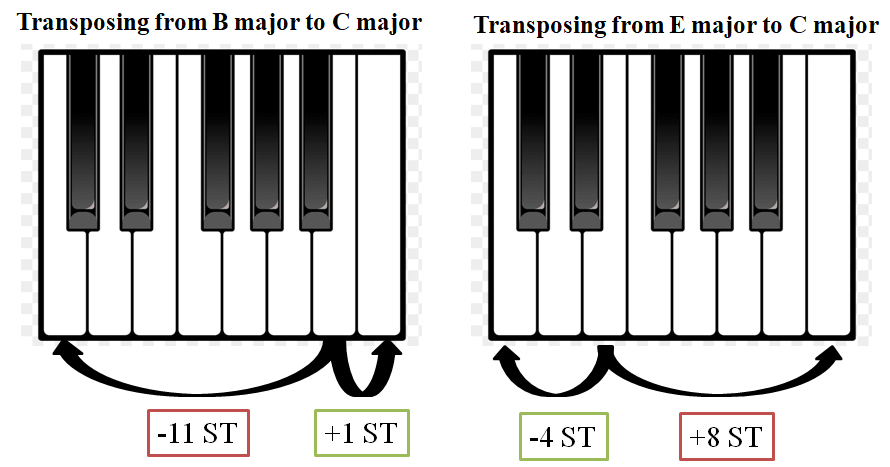
\includegraphics[width=0.9\textwidth]{transposing2.png} % Adjust width
    \caption{The Transposition Problem, optimal solution green}
    \label{fig:transp}
\end{figure}

\begin{lstlisting}
def transpose_midi(pretty_midi_stream, interval):
#Author: Julian Napier
    # Transpose the MIDI using pretty_midi
    transposed_midi = pretty_midi.PrettyMIDI()

    # Loop over all instruments and transpose their notes
    for instrument in pretty_midi_stream.instruments:
        transposed_instrument = pretty_midi.Instrument(instrument.program, is_drum=instrument.is_drum)
        for note in instrument.notes:
            transposed_note = pretty_midi.Note(
                velocity=note.velocity,
                pitch=note.pitch + interval,
                start=note.start,
                end=note.end
            )
            transposed_instrument.notes.append(transposed_note)
        transposed_midi.instruments.append(transposed_instrument)

    return transposed_midi
\end{lstlisting} 
Now, once we know our transpose interval, we can now perform the actual transposition in pretty\_midi, with the transpose interval as an argument (line 1). This is fairly straight forward: First we create a target file that we will return (line 4). Then we loop through all instruments of the old file (drums are already filtered out), create a new instrument and add the same notes with the semitones to transpose added onto their pitch (lines 8-16). This instrument we then append to the target file (line 17).

\subsubsection{Making Monophonic}
Making our training input monophonic is essential for hook generation. Only this way, the transformer can focus on the core melody and not get distracted by harmonies. \newline

\begin{figure}[H] % 'h' means here
    \centering
    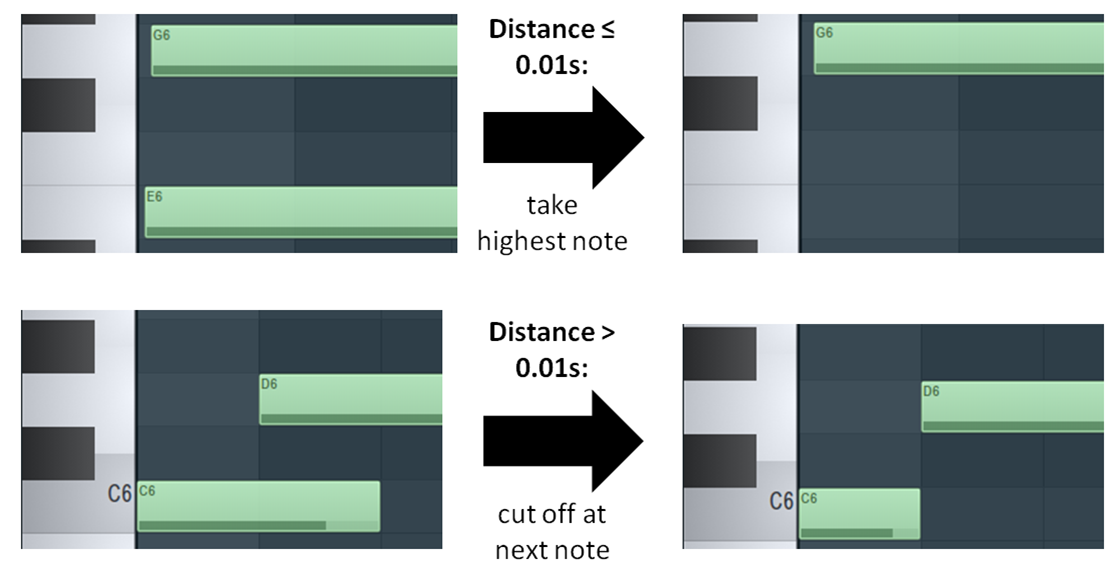
\includegraphics[width=0.9\textwidth]{monophonic.png} % Adjust width
    \caption{Different Approaches For Making Monophonic}
    \label{fig:mon}
\end{figure}

To achieve this task, we need to make the following differentiation: For one, if a chord is being played, we want to take the top note. If a melody is being played, it could potentially overlap with other notes. To fix this, we want to cut off the old note when the new note starts. When to do which of these is decided by a time tolerance parameter (line 10), in our case 0.01 seconds. This is illustrated in Figure \ref{fig:mon}. \newline

\begin{lstlisting}
def make_monophonic(pretty_midi_stream): #Author: Julian Napier
    for instrument in pretty_midi_stream.instruments:
        # Sort notes by start time
        instrument.notes.sort(key=lambda note: note.start)
        # Prepare a new list to store monophonic notes
        monophonic_notes = []
        # Initialize a list to track simultaneous notes
        chord_group = []
        # Tolerance for identifying simultaneous notes (in seconds)
        time_tolerance = 0.01

        # Process notes
        for note in instrument.notes:
            # If the chord group is empty, add the first note
            if not chord_group:
                chord_group.append(note)
            else:
                # If the current note starts within the time tolerance of the first note in the group, add to chord
                if abs(note.start - chord_group[0].start) <= time_tolerance:
                    chord_group.append(note)
                else:
                    # Process the chord group to keep only the highest note
                    top_note = max(chord_group, key=lambda n: n.pitch)
                    # If overlap occurs, cut the previous note's end time
                    if monophonic_notes and monophonic_notes[-1].end > top_note.start:
                        monophonic_notes[-1].end = top_note.start
                    # Add the highest note to the monophonic list
                    monophonic_notes.append(top_note)
                    # Start a new chord group with the current note
                    chord_group = [note]

        # Handle the last chord group
        if chord_group:
            top_note = max(chord_group, key=lambda n: n.pitch)
            # Adjust overlap for the last group
            if monophonic_notes and monophonic_notes[-1].end > top_note.start:
                monophonic_notes[-1].end = top_note.start
            monophonic_notes.append(top_note)

        # Replace the instrument's notes with the monophonic notes
        instrument.notes = monophonic_notes
\end{lstlisting}
All in all, the function loops through all tracks and performs the task separately on each track/instrument (line 2). First we sort the notes by their start time (line 4). Then we prepare different data structures: chord\_group (line 8) for notes within the time tolerance, monophonic\_notes (line 6) for the end result. Then the actual processing starts. We go through each note in the current track (line 13) and do the following: If there is no note in chord\_group, we add the current note (line 16). Otherwise we check whether the current note is within the time tolerance of the first note in the chord (line 19). If yes, we append the note to the chord group (line 20). If no, we take the highest note and append it the our result (line 28), fixing any occuring overlaps (line 26). After that, we start a new chord group with the current note, since it didn't belong to the previous chord. After looping through all notes, we still might have notes in chord\_group. This we handle in lines 32-38, analogously. In the end, we replace the tracks notes with our monophonic result (line 41).



\subsubsection{The Collection Method}
\begin{lstlisting}
def greedy_collect(pretty_midi_stream, tempo, output_path_pref):
#Author: Julian Napier
    tracks_coll = 0
    tracks_skipped = 0
    for i, instr in enumerate(pretty_midi_stream.instruments):
        if instr.notes: #this might be this case with removed bass tracks f.e.
            midi = pretty_midi.PrettyMIDI(initial_tempo=120) #create a new midi file for writing
            seconds_per_beat = 60.0 / tempo
            seconds_per_bar = 4 * seconds_per_beat #4 beats in one bar (4/4, we treat 2/4 just like 4/4 here)
            bar_duration = seconds_per_bar * 8  # Duration of 8 bars in seconds

            first_note_time = min(note.start for note in instr.notes) 

            cutoff_time = first_note_time + bar_duration #cutoff point 8 bars after first note

            new_instrument = pretty_midi.Instrument(program=instr.program, is_drum=instr.is_drum)
            new_instrument.notes = [note for note in instr.notes if first_note_time <= note.start < cutoff_time] #notes in 8 bars from first note

            bars = [[] for _ in range(8)]

            for note in new_instrument.notes:
                # Find the bar index (0-based index for 8 bars)
                bar_index = int((note.start - first_note_time) // seconds_per_bar)
                if 0 <= bar_index < 8:  # Ensure it's within the 8 bars
                    bars[bar_index].append(note)

            bars_with_notes = sum(1 for bar in bars if len(bar) > 0)

            if bars_with_notes >= 6: #something must be played in at least 6 out of 8 bars
                for note in new_instrument.notes:
                    note.start = max(0, note.start - first_note_time)
                    note.end = max(0, min(note.end - first_note_time, cutoff_time - first_note_time))
                    note.start *= tempo/120 #Stretch to 120 bpm from original tempo
                    note.end *= tempo/120
                if len(new_instrument.notes) >= 12: #there must be at least 12 notes in file
                    midi.instruments.append(new_instrument)
                    op_new = str(output_path_pref) + f"_track{i}.mid"
                    midi.write(str(op_new))
                    #print(f"8 bar excerpt saved to: {op_new}")
                    tracks_coll += 1
                else: tracks_skipped += 1
            else: tracks_skipped += 1

    return tracks_coll, tracks_skipped
\end{lstlisting}
This function handles steps 5-7 of the algorithm.
After initializing counters (lines 3, 4) , we iterate through all remaining tracks/instruments that still have notes (lines 5, 6). For each of them, we create a target file in 120 bpm (line 7). We calculate the seconds pear beat and bar considering the original tempo (lines 8, 9), which was given to the function as a parameter. From these results we then calculate the length of 8 bars (line 10). After that, we compute the time when the first note starts and the time where the 8 bar phrase should end (lines 12, 14). We then create an instrument with the notes from the 8 bars after the first note is played (lines 16, 17). Then we create a list of 8 lists for each bar, which we fill with the corresponding notes by using integer division (lines 19-25). After that, we calculate how many bars have notes (line 27). This we use to check one of our note density criteria (line 29). If this criterion is met, we shift the note start and end times so that the first note starts at the beginning of the sequence and not somewhere else, respecting all edge cases (lines 31, 32). 
After doing that we stretch all note start and end times by a factor of tempo/120 to actually be in 120 bpm (lines 33, 34). This is necessary because we imported the notes in to a 120 bpm track, even though there were still in the original tempo of the song. Next we check our second note density criterion (line 35). If it is met, we append the created instrument to a MIDI file and write it (lines 36-40). If either criterion isn't met, we skip the track/instrument (lines 41, 42). In the end we return some counters for statistics (line 44).


\subsection{Evaluation}
\subsubsection{Collection Statistics}

When running our algorithm on the clean MIDI subset, we received the following statistics:
\begin{comment}
\lstset{style=allblack}
\begin{lstlisting}
17256 files processed.
Removed 0 midi files due to non-major/minor mode.
Skipped 6846 files in total due to time signature.
Skipped 6846 files in total.

37385 8 bar excerpts collected.
Removed 16651 drum tracks in total.
Removed 19392 bass tracks in total.
Skipped 25012 tracks in total due to note density.
Skipped 61055 tracks in total.
\end{lstlisting}
\lstset{style=mystyle}
\end{comment}
\begin{figure}[H]
    \centering
    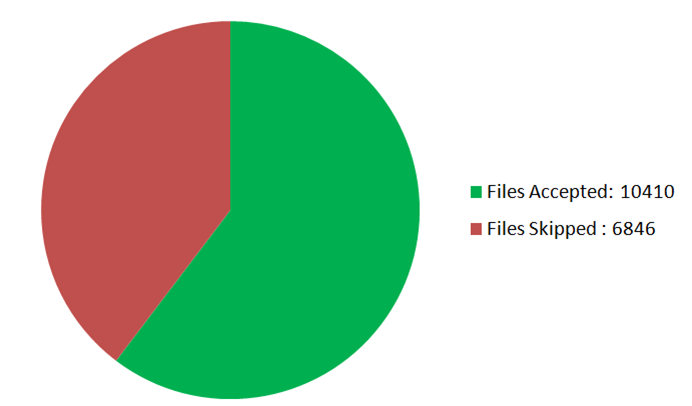
\includegraphics[width=0.7\textwidth]{fileproc.png}
    \caption{File Processing Statistics}
    \label{fig:tproc}
\end{figure}

The clean MIDI subset contains 34518 files, 17526 of these were able to be processed without an error. In total, 6846 out of these 17526 files (39.7\%) were skipped due to time signature or tempo. No files were skipped due to a non-major/minor mode.

\begin{figure}[H]
    \centering
    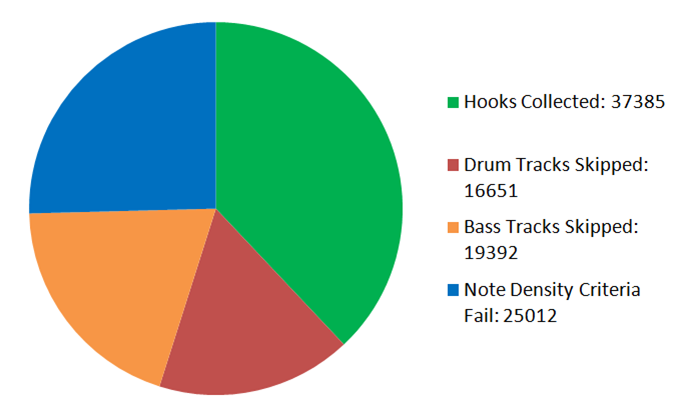
\includegraphics[width=0.7\textwidth]{trackproc.png}
    \caption{Track Processing Statistics}
    \label{fig:fproc}
\end{figure}

In total, 98440 tracks were processed. We collected hooks from 37875 (38\%) of these. 16651 (16.9\%) drum tracks were skipped. 19392 (19.7\%) suspected bass tracks were skipped. 25012 (25.4\%) were skipped because the first 8 bars after the first played note didn't fulfill our note density criteria.

\subsubsection{Positive/Negative Examples}
In this section we will list some positive and negative results from our Hook Collection. As a test set we used ABBA songs. The corresponding MIDI files can be found in ... \newline

\textit{Positive Examples:}

\begin{itemize}
    \item In "Dance (While the Music Still Goes on)1\_track0" the vocal hook from the beginning is captured well.
    \item In "Mamma Mia\_track0" the piano hook from the intro is captured perfectly.
    \item In "Name of the Game.1\_track4" a nice accompanying string melody is captured.
    \item In "Name of the Game.1\_track8" an vocal interesting accompaniment arppegio is captured.
    \item In "Summer Night City\_track4" a minimalistic, but good hook is captured.
\end{itemize}

\textit{Negative Examples:}

\begin{itemize}
    \item In "Dance (While the Music Still Goes on).1\_track6" the top note from a chord accompaniment is captured. It sounds fine, but isn't a great hook
    \item In "I Do, I Do, I Do, I Do\_track1" once again top notes from a chord accompaniment are captured, that don't sound like a hook on their own.
    \item In "Just Like That (Full Sax version) (1983)\_track1" a rhythmic accompaniment that sounds monotonic and bland is captured.
    \item In "Opus 10\_track1" the rhythm and notes seem a little random, not catchy at all.
    \item In "The Living Daylights\_track16" a interesting rhythm is captured. However, the pattern mostly alternates between two notes, which is a bit boring.
\end{itemize}



\subsubsection{Potential Improvements}

On file level, filtering out files with alternating time signatures and tempo and focusing on 4/4 time signature is definitely an important step toward uniformity.
On track level drum track skipping, tranposing and making monophonic also worked very well.
However, the next steps of our algorithm can be questioned: \newline

First of all, skipping tracks with notes lower than F2 after steps 2 and 3 gets rid
of more tracks than it actually should; as can be seen in "Collection Statistics",
about every fifth track is classified as a bass track, even though every file usually has 6 or more tracks, only one of them being a bass track.
This could be solved by training a classifier (Binary Logistic Regression, Neural Network or Transformer) to detect whether a track is a bass track or not.
Another possibly useful feature is that bass tracks are always monophonic. Tracks that aren't monophonic (before making everything monophonic) are therfore definitely never a bass track and wouldn't have to be skipped. \newline

Secondly, the approach of cutting out 8 bars after the first played note in a so far accepted track isn't the best solution.
It ignores the fact that a better hook could theoretically could be in the middle of the track. 
Another approach would be slicing the input into 8 bar pieces after the first played note and checking certain note density criteria for each.
This would have the advantage that more data is collected and the disadvantage that many 8 bar sequences wouldn't be hooks, since songs also have a lot of other melodies.
Another possibility without this disadvantage would be to training a neural network to predict the 8 bars most likely to be a hook in a MIDI sequence and then collecting that. \newline

And thirdly, our note density criteria are rather strict. It can be argued that a note played in 4 or 5 out of 8 bars would suffice.
However, at the with those settings we generated a lot of pauses and this was an easy and effective way for us to counteract this.


\section{Tokenization}
\subsection{The REMI Tokenizer}
In order to tokenize our midi events we use the REMI tokenizer, implemented in the miditok (\cite{miditok2021}) library, which was first introduced in the Pop Music Transformer paper written by \cite{huang_remi_2020}. The REMI tokenizer provides a structured approach to representing musical events in MIDI format by breaking down the sequence of notes into a series of tokens. This tokenization method captures essential musical features such as Bar, Pitch and Note Duration. Therefore it is well fit for our task.

\subsection{Important Configuration Parameters}
\begin{lstlisting}
    TOKENIZER_PARAMS = {
        "pitch_range": (21, 109),
        "beat_res": {(0, 32): 8},
        "num_velocities": 1,
        "special_tokens": ["PAD", "BOS", "EOS"],
        "use_note_duration_programs": [-1, 0, 1, 2, 3, 4, 5, 6, 7, 8, 9, 10, 11, 12, 13, 14, 15, 16, 17, 18, 19, 20, 21, 22, 23, 24, 25, 26, 27, 28, 29, 30, 31, 32, 33, 34, 35, 36, 37, 38, 39, 40, 41, 42, 43, 44, 45, 46, 47, 48, 49, 50, 51, 52, 53, 54, 55, 56, 57, 58, 59, 60, 61, 62, 63, 64, 65, 66, 67, 68, 69, 70, 71, 72, 73, 74, 75, 76, 77, 78, 79, 80, 81, 82, 83, 84, 85, 86, 87, 88, 89, 90, 91, 92, 93, 94, 95, 96, 97, 98, 99, 100, 101, 102, 103, 104, 105, 106, 107, 108, 109, 110, 111, 112, 113, 114, 115, 116, 117, 118, 119, 120, 121, 122, 123, 124, 125, 126, 127],
        "use_chords": False,
        "use_rests": True,
        "beat_res_rest": {(0, 32): 8},
        "use_tempos": False,
        "use_time_signatures": False,
        "time_signature_range": {4: [4]},
        "use_programs": False,
        "use_pitchdrum_tokens": False,
        "default_note_duration" : 0.5, 
        "num_tempos": 32,  # number of tempo bins
        "tempo_range": (120, 120),  # (min, max)
        "encode_ids_split": 'no',
        "ac_note_duration_track": True,
        "ac_note_density_track": True,
        "ac_repetition_track": True,
        "ac_repetition_track_num_bins": 8
    }
\end{lstlisting}
These are the configuration parameters we used to set up our tokenizer. They can be found in \textit{Transformer\_Code/CUPY/models/utils/generate\_tokenizer.py}. Many are default settings, but some of them we had to adapt to our task:\newline
\begin{lstlisting}
"beat_res": {(0, 32): 8}   
\end{lstlisting}
This setting enables the tokenizer to capture notes up to 32nd notes in the first 8 bars (these are equal to 32 beats, our inputs are never longer than this). Notes in between are rounded to the nearest 32nd note. We chose 32nd notes because in popular music notes are rarely shorter than this. \newline
\begin{lstlisting}
"num_velocities": 1
\end{lstlisting}
We don't care about different velocities in melodies, since these have nothing to do with the notes played. That's why we downsample everything to have the same velocity. \newline

\begin{lstlisting}
"use_chords": False
\end{lstlisting}
Since our input is monophonic, there are no chords, so we don't want the tokenizer to try and encode them. \newline

\begin{lstlisting}
"use_rests": True,
"beat_res_rest": {(0, 32): 8}
\end{lstlisting}
Rests are important to capture the rhythm of the hooks correctly. That's why we capture them at the same beat resolution as played notes. \newline

\begin{lstlisting}
"use_tempos": False,
"tempo_range": (120, 120),
"use_time_signatures": False,
"time_signature_range": {4: [4]}
\end{lstlisting}
These settings align with how we collected our data. We can treat everything as a 120 bpm, 4/4 time signature hook. Any different time signatures or tempos aren't needed. \newline

\begin{lstlisting}
"encode_ids_split": 'no'
\end{lstlisting}
The default setting here was 'bar', meaning that tokens weren't able to go beyond bars. This is problematic, since important melodic structures and repetitions of hooks do go beyond bars, that's why we set this parameter to 'no'. \newline

\begin{lstlisting}
"ac_note_duration_track": True,
"ac_note_density_track": True,
"ac_repetition_track": True,
"ac_repetition_track_num_bins": 8
\end{lstlisting}
These parameters allow the tokenizer to use extra tokens to track certain behaviours in our hooks like note duration (important for capturing rhythm correctly), repetition (very important in hooks due to the repetitiveness) and note density development.
In monophonic melodies, only one note is active at a time, so the vocabulary doesn’t need to account for simultaneous note combinations (e.g., chords).
We opted for a vocabulary size of 4096 which might be very generous given that out data consists of single-note melodies.
In addition to that we expect short sequences: An 8-bar melody is relatively short, especially in monophonic form. For example, in 4/4 time at 120 BPM, an 8-bar melody lasts 16 seconds.

\subsection{Data Augmentation}
In order to enlarge our training data we choose to augment the midi tracks by shifting the melody one octave up, two octaves up, one octave down and two octaves down. Fortunately the MidiTok library already built a data augmentation function which we used in our project.
\subsection{Token Statistics}
\label{sec:token_stats}
In this section we summarise the tokenization procedure by showing distributional information. \newline

Firstly we observed that the top 20 tokens are all tokens which encode Tempo events.
REMI insert tempo tokens at regular intervals (e.g., every bar or every beat) to ensure the timing information is preserved.
We opted for capturing a 32nd note resolution and therefore many Tempo tokens are used in order to capture this granulated beat resolution.
Figure (\ref{fig:token_distribution}) depicts the total token distribution. The top 20 token are responsible for the spike at around 350. Starting from token 696 we observed token ids which actually encode Note events. These are responsible for the second peak which flattens out.
It is important to note that the Note Events do also encode time, duration, pitch and velocity. In total the vocabulary has 2955 tokens for Note events and 1141 tokens for Tempo events.

With regard to the sequence length distribution we see that 50\% of the input files have a sequence length smaller than 103.
Nevertheless the variance of sequence lengths is quite high as seen in Figure (\ref{fig:log_seq_len}) and (\ref{fig:cumulative_seq_len}). We used this information to choose the models context size which is discussed in section \ref{sec:Training}. \newline
\begin{figure}[H]
    \centering
    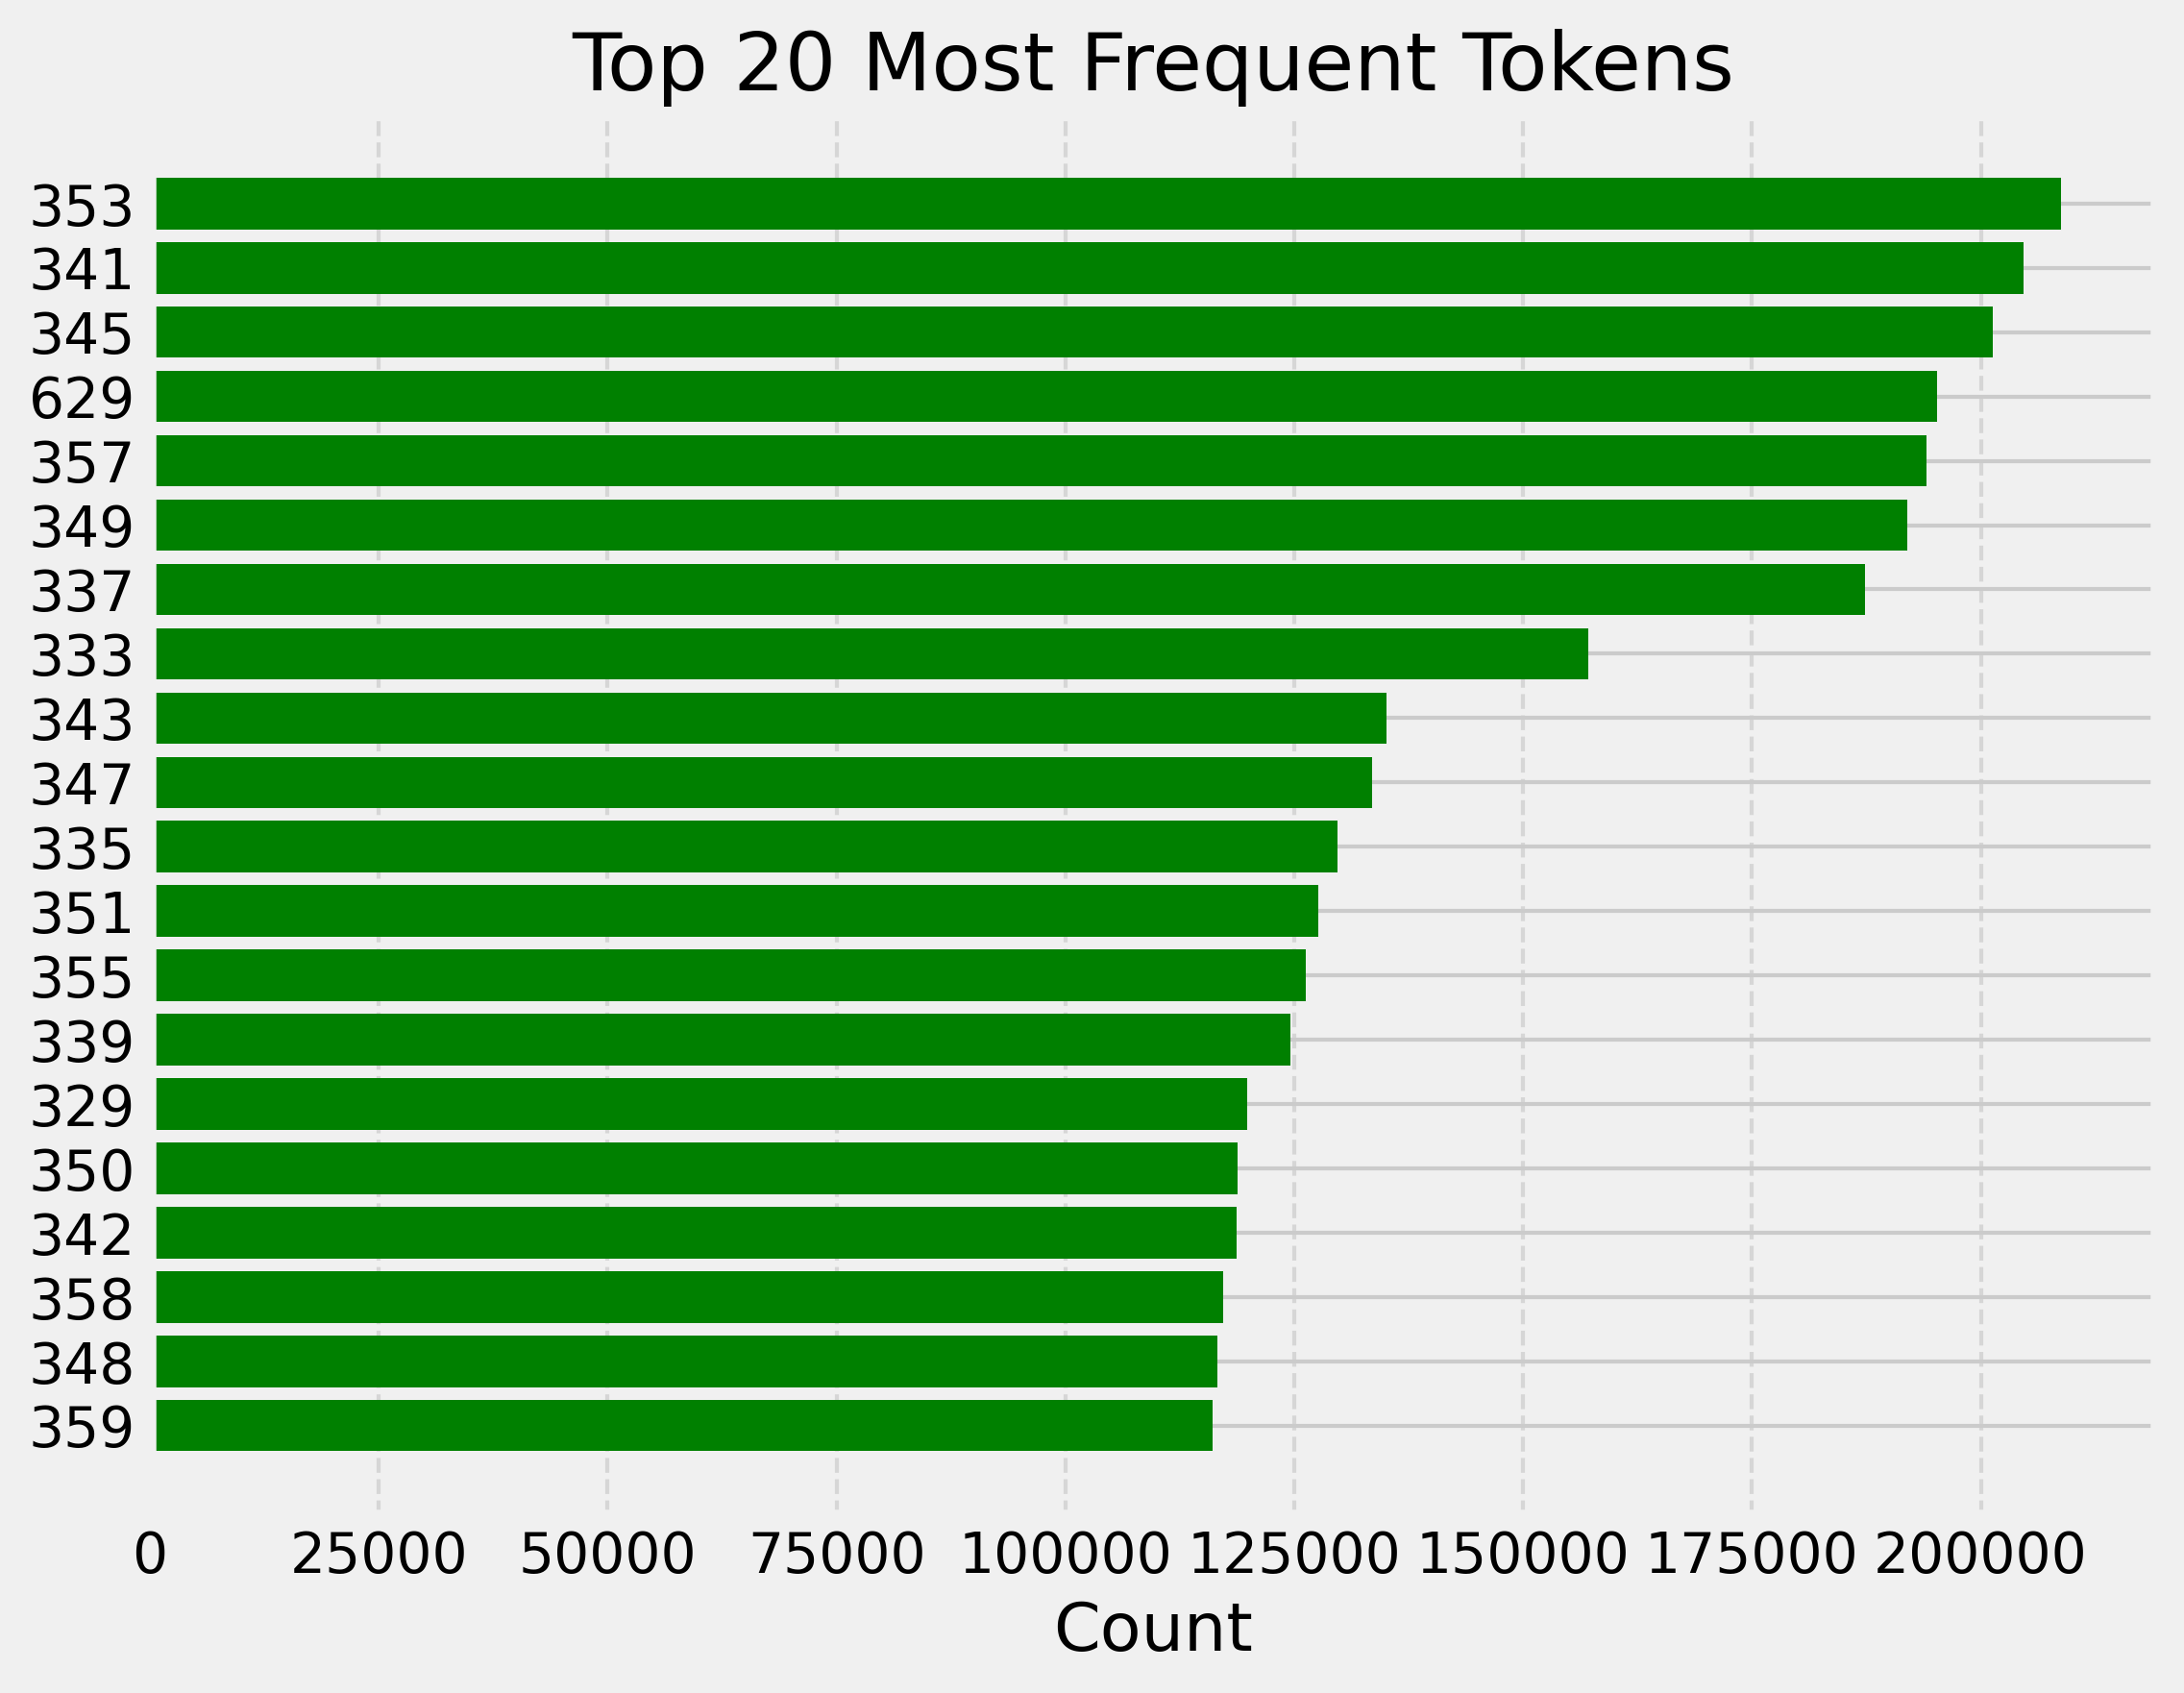
\includegraphics[width=0.65\textwidth]{visualization_4096_REMI_train_manual_tokens_True_random_padding_True_top_frequent_tokens.png}
    \caption{Top 20 tokens}
    \label{fig:top_20_tokens}
\end{figure}

\begin{figure}[H]
    \centering
    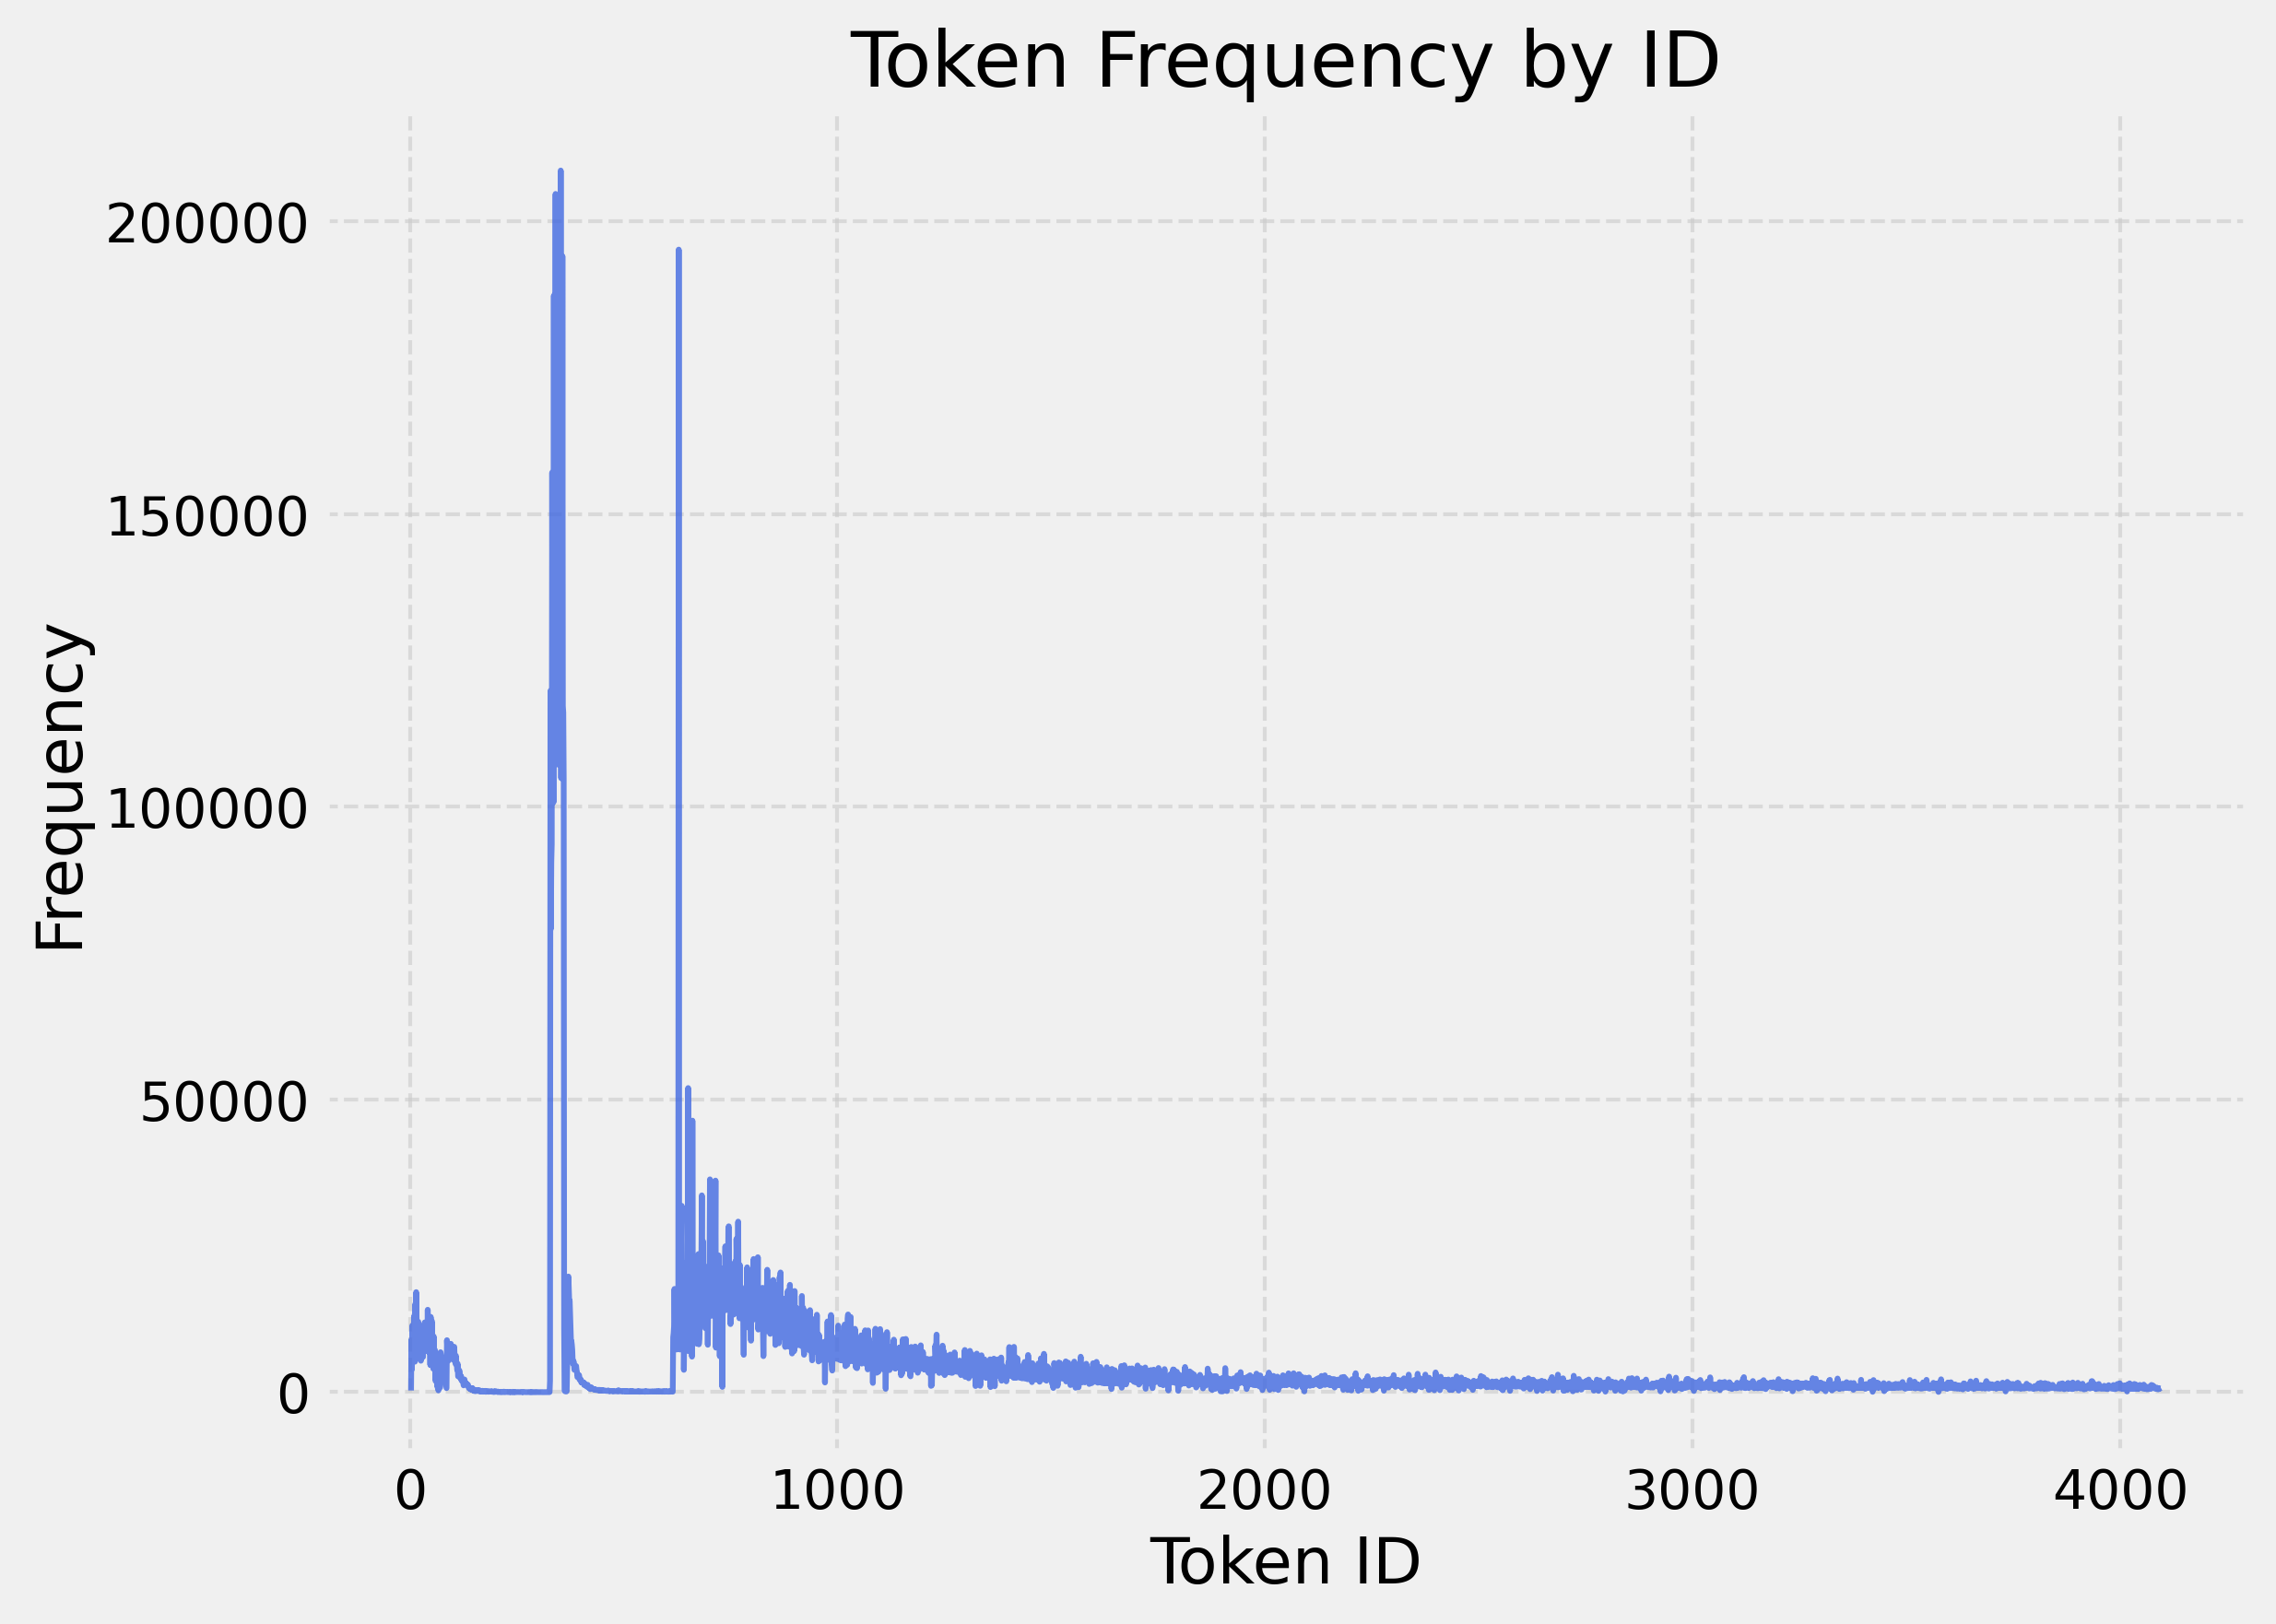
\includegraphics[width=0.65\textwidth]{visualization_4096_REMI_train_manual_tokens_True_random_padding_True_token_frequency_by_id.png}
    \caption{Token distribution}
    \label{fig:token_distribution}
\end{figure}

\begin{figure}[H]
    \centering
    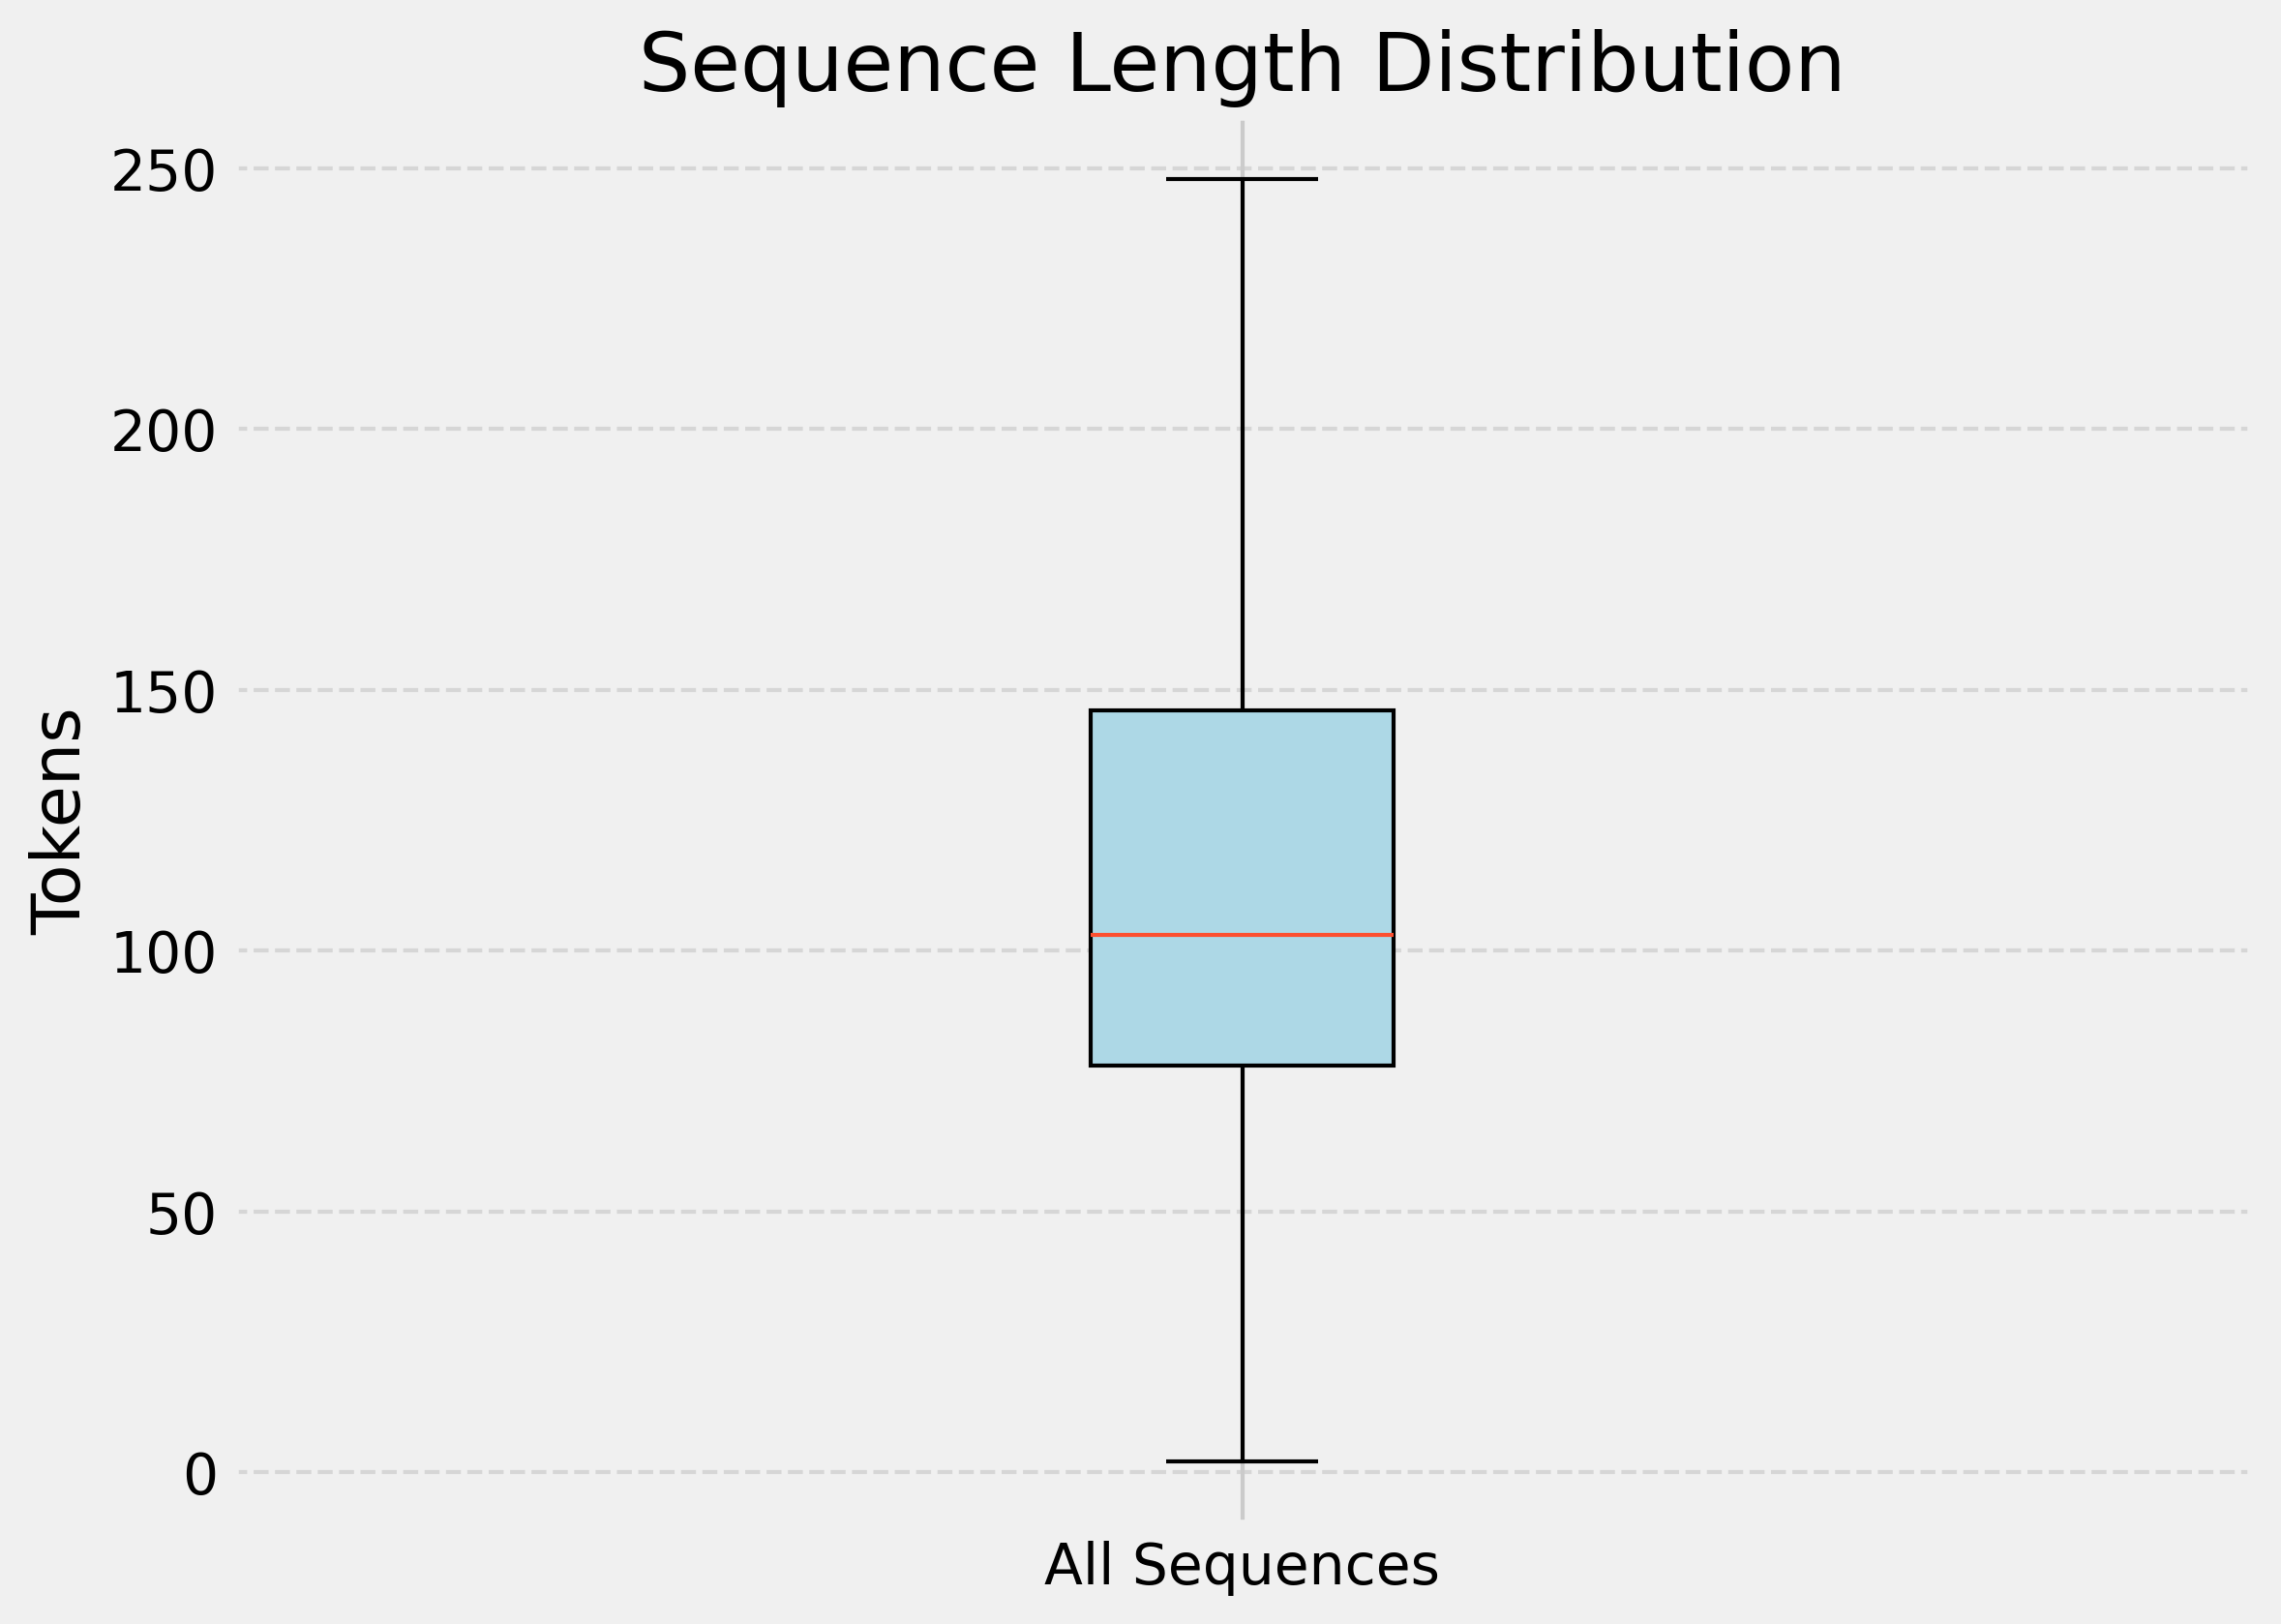
\includegraphics[width=0.65\textwidth]{seq_len_box_plot.png}
    \caption{Sequence Length Box Plot}
    \label{fig:seq_len_box_plot}
\end{figure}
\begin{figure}[H]
    \centering
    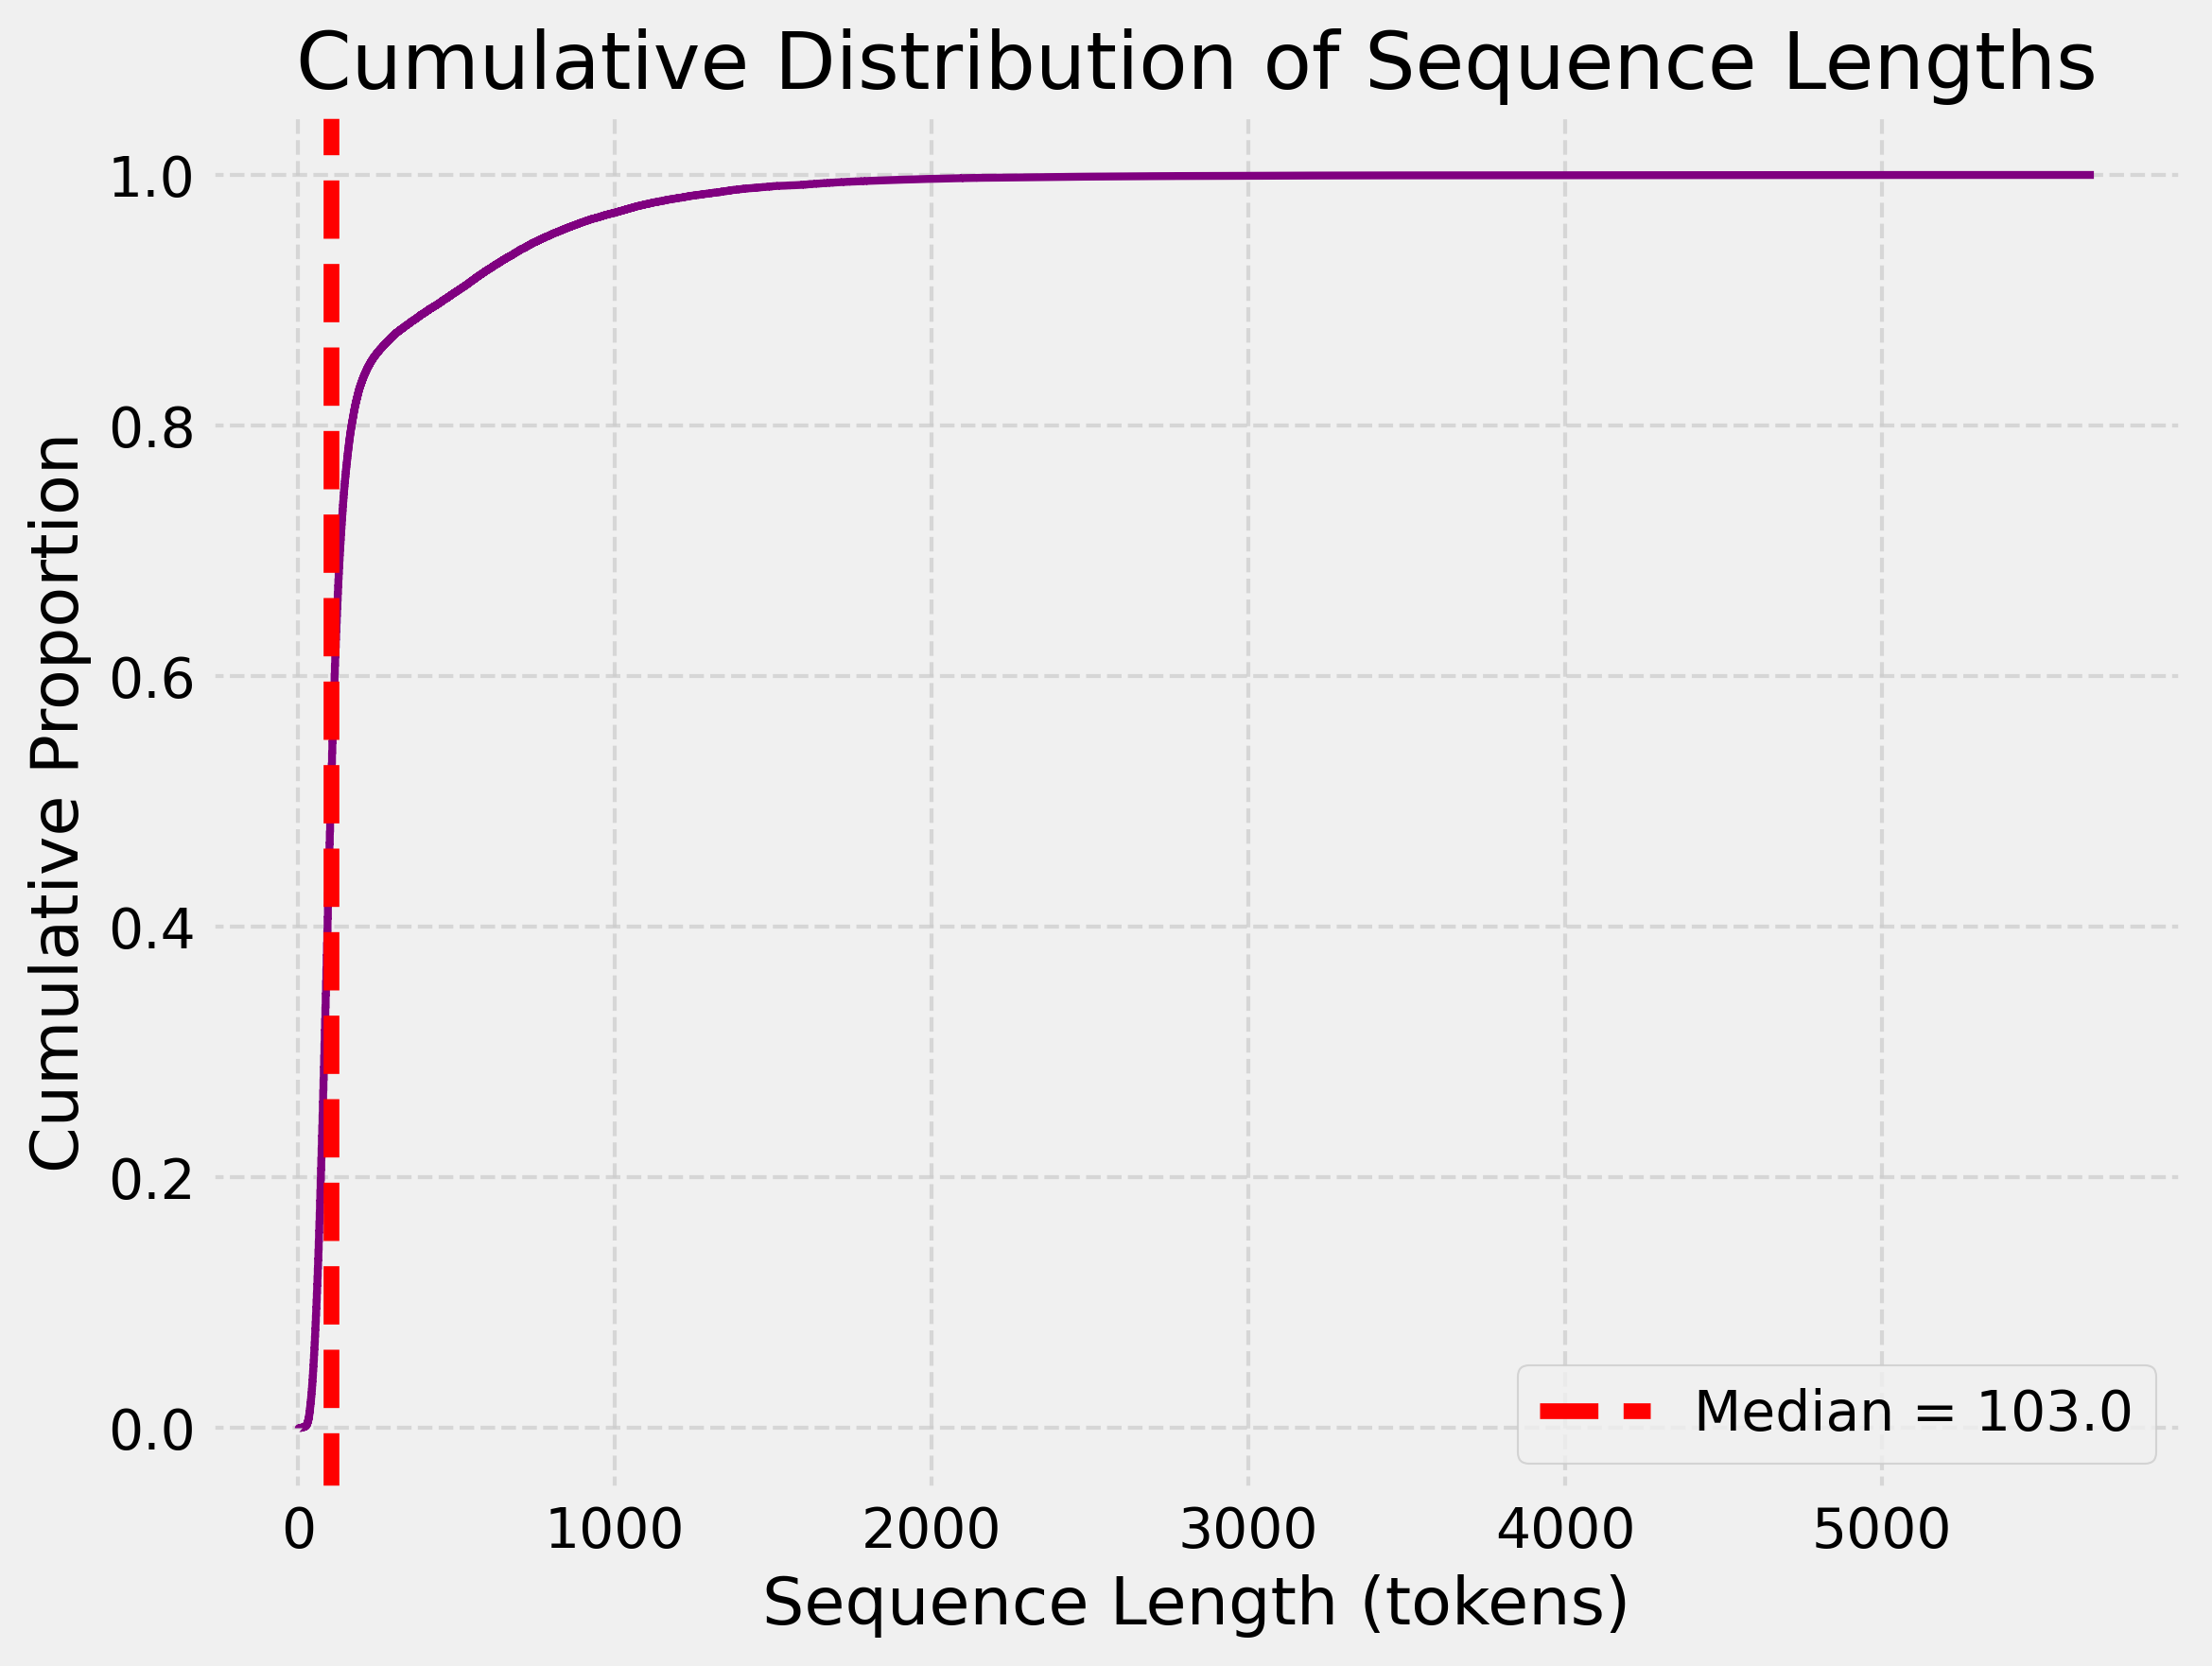
\includegraphics[width=0.65\textwidth]{visualization_4096_REMI_train_manual_tokens_True_random_padding_True_cumulative_length_distribution.png}
    \caption{Cumulative Distribution of Sequence Lengths}
    \label{fig:cumulative_seq_len}
\end{figure}

\begin{figure}[H]
    \centering
    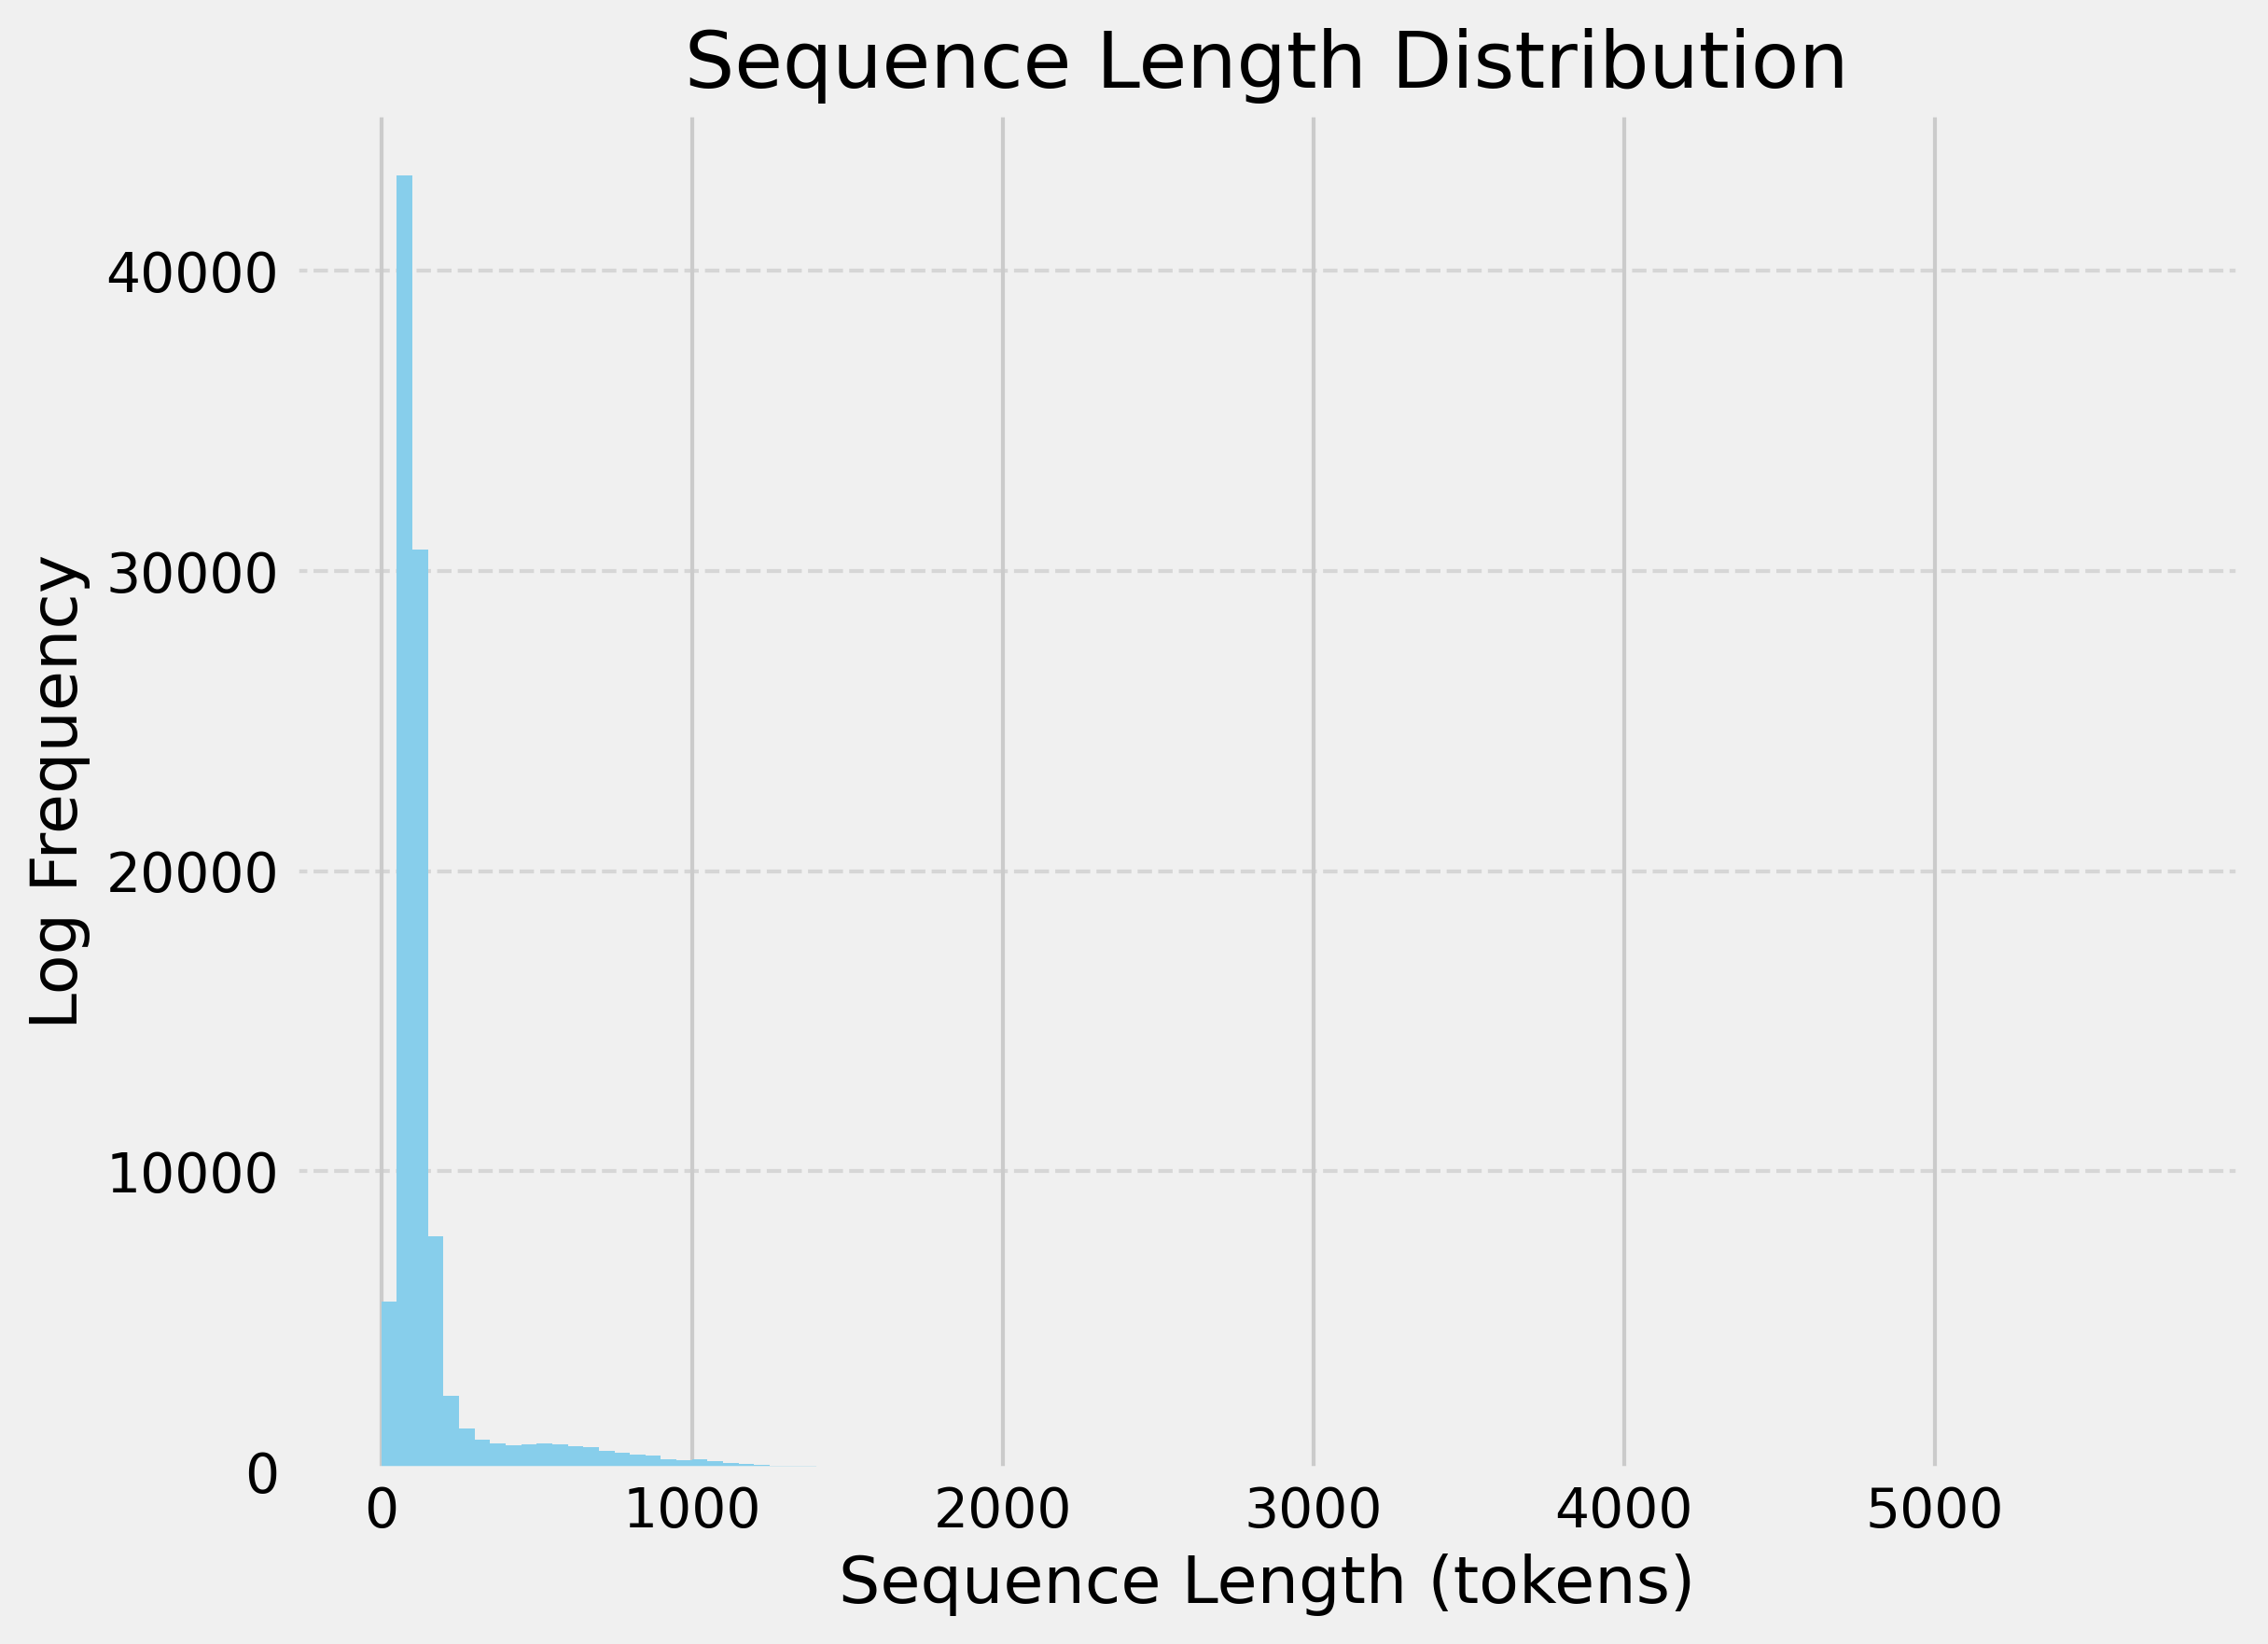
\includegraphics[width=0.65\textwidth]{visualization_4096_REMI_train_manual_tokens_True_random_padding_True_seq_length_distribution.png}
    \caption{Log Distribution of Sequence Lenghts}
    \label{fig:log_seq_len}
\end{figure}


\section{Relative Attention}
\subsection{Overview}

\textit{Note: As an abbreviation for the matrix dimensions we will be using B for the batch size, H for the number of heads, L for the sequence length and D for the head depth.} \newline

Since we are dealing with music in this task, the Absolute Attention mechanism commonly used in transformers \parencite{DBLP:journals/corr/VaswaniSPUJGKP17} doesn't quite cut it. This mechanism only captures the relationship of tokens at absolute positions with one another. However, we also need to capture general relationships between notes. For example: How do adjacent notes/tokens correlate in general, can we infer anything from our data? \newline

A solution to this problem was first introduced by \textcite{shaw2018selfattentionrelativepositionrepresentations} and then refined by \textcite{DBLP:journals/corr/abs-1809-04281}. The main objective is to capture these relationships in the form of learnable relative positional embeddings $E$ (of dimensions $1 \times H \times L \times D$) in every attention block. Each row of such a matrix corresponds to a certain key-query distance, as can be seen in Figure \ref{fig:relatt}. 
\newline

\begin{figure}[H] % 'h' means here
    \centering
    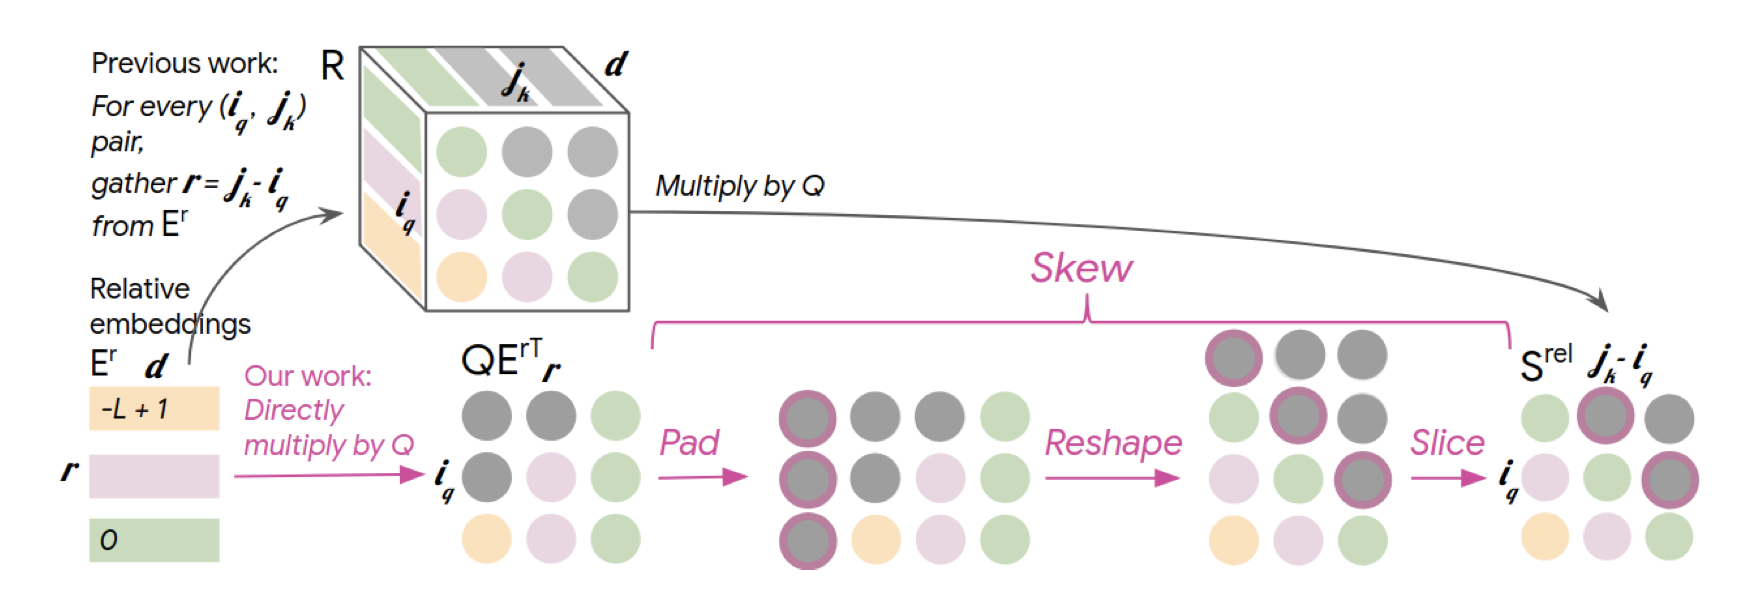
\includegraphics[width=0.9\textwidth]{relative_attn_skewing.png} % Adjust width
    \caption{Relative Attention With Skewing, \textcite{DBLP:journals/corr/abs-1809-04281}}
    \label{fig:relatt}
\end{figure}
\vspace{0.1cm}
The first step of the attention process is to multiply $Q$ by $E^T$, resulting in a matrix of dimensions $B \times H \times L \times L$ ($E$ is broadcasted over $B$ beforehand). Its $(i_q, r)$ entry contains the dot product of the query in position $i_q$ with the embedding of relative distance $r$. However, each relative logit $(i_q, j_k)$ in the matrix $S_\text{rel}$  should be the dot product of the query in position $i_q$ and the corresponding key $j_k$ with relative distance $r$, to match up with the indexing in $QK^T$.
\textcite{DBLP:journals/corr/abs-1809-04281} propose the "skewing" algorithm to move the relative logits of $QE^T$ to their correct positions, as illustrated in Figure \ref{fig:relatt}:

\begin{enumerate}
\item Pad a dummy column vector before the leftmost column (shape: $B$, $H$, $L$, $L + 1$).
\item Reshape the matrix to have shape ($B$, $H$, $L + 1$, $L$).
\item Discard the top row of the third dimension (shape: $B$, $H$, $L$, $L$).
\end{enumerate}

The result of this process is the relative attention score matrix $S_\text{rel}$ with correct indexing, as outlined in Equation (1). This matrix is now added to the conventional attention scores $QK^T$. This sum then goes through the normal attention process from \textcite{DBLP:journals/corr/VaswaniSPUJGKP17}, as outlined in Eq. 2.\vspace{0.15cm}
\begin{align}
S_{\text{rel}} &= \text{skew}(QE^T) \\[0.2cm] 
\text{RelativeAttention} &=
\text{softmax}\left(\frac{QK^T+S_\text{rel}}{\sqrt{d_k}}\right)V
\end{align}

\subsection{Implementation}
\subsubsection{Forward Pass}
In this section, we will go through all relevant differences to normal Absolute Attention in the Forward Pass, meaning we won't be showing any computations that are exactly the same as in Absolute Attention. All code for this and the next subsection can be found in \textit{Transformer\_Code/CUPY/models/GoePT/layers.py}\newline
\begin{lstlisting}
    self.x1 = q @ e.transpose(0, 1, 3, 2) #Q * E_T
\end{lstlisting}
Here we compute $X_1 = QE^T$ as portrayed in the section "Overview", the broadcasting of $E$ happens automatically here.\newline
\begin{lstlisting}
    self.x2 = cp.pad(self.x1, ((0, 0), (0, 0), (0, 0), (1, 0)), mode='constant', constant_values=0) #padding, adding a column of zeros to the left of the T x T matrix, results in (B, nh, T, T + 1)
\end{lstlisting}
Step 1 of the Skewing Algorithm: \( X_2 = \text{pad\_left\_column}(X_1) \).\newline

\begin{lstlisting}
    self.x3 = self.x2.reshape(B, self.n_heads, T + 1, T) #reshape to (B, nh, T + 1, T) matrix
\end{lstlisting}
Step 2 of the Skewing Algorithm: \( X_3 = \text{reshape } X_2\) to ($B$, $H$, $L + 1$, $L$). \newline

\begin{lstlisting}
    self.s_rel = self.x3[:, :, 1:, :] #discard first row of 3rd dim, new dim: (B, nh, T, T)
\end{lstlisting}
Step 3 of the Skewing Algorithm: \( S_\text{rel} = \text{discard\_top\_row}(X_3)\)\newline

\begin{lstlisting}
    attn = (q @ k.transpose(0, 1, 3, 2) + self.s_rel)*(1.0/math.sqrt(k.shape[-1])) #relative attention
\end{lstlisting}
Here we implement the mask input from Equation 2 from the section "Overview". From here on everything works exactly the same as in Absolute Attention.


\subsubsection{Backward Pass}
\textit{Note: We will be using $M = \frac{QK^T+S_\text{rel}}{\sqrt{d_k}}$ as an abbreviation for the mask input from Equation (2). In addition, we will be using $E_b$ as an abbreviation for $E$ broadcasted to all batches. We also implicitly assume that transposition and matrix multiplication only happen over the last two dimensions of tensors. Therefore we will be referring to the the 3rd dimension as rows and 4th dimension as columns.}\newline

In this section, we will go through all relevant differences to Absolute Attention in the Backward Pass, so we won't be showing gradients that are exactly the same. $\frac{\partial L}{\partial M}$ is already given to us, since the attention process after computing M is identical to the process in absolute attention (first mask, then softmax etc.).\newline

\begin{lstlisting}
    grad_s_rel = (1.0/math.sqrt(self.k.shape[-1])) * grad_mask
\end{lstlisting}
\begin{align}
\frac{\partial L}{\partial S_\text{rel}}
&= \frac{\partial L}{\partial M} \cdot \frac{\partial M}{\partial S_\text{rel}} \\[0.15cm]
&= \frac{\partial L}{\partial M} \cdot \frac{1}{\sqrt{d_k}}
\end{align}

\raggedright The gradient of $L$ with respect to $S_\text{rel}$ can be easily computed with the chain rule (Eq. 3). The gradient of $M$ with respect to $S_\text{rel}$ is simply the constant $\frac{1}{\sqrt{d_k}}$ (Eq. 4). \newline
\vspace{0.1cm}
\begin{lstlisting}
    grad_x3 = cp.pad(grad_s_rel, ((0, 0), (0, 0), (1, 0), (0, 0)), mode='constant', constant_values=0) #pad top row
\end{lstlisting}
\begin{align}
\frac{\partial L}{\partial X_3}&=\text{pad\_top\_row}\left(\frac{\partial L}{\partial S_\text{rel}}\right)
\end{align}

The gradient of $L$ with respect to $X_3$ can be received by performing the reverse operation of step 3 of the Skewing Algorithm. There we discarded the top row, now we pad the top row of our current gradient $\frac{\partial L}{\partial S_\text{rel}}$ with 0's (Eq. 5). This results in a tensor of shape $(B, H, L + 1, L)$. \newline
\vspace{0.1cm}

\begin{lstlisting}
    grad_x2 = grad_x3.reshape(B, self.n_heads, T, T + 1) #reverse reshaping
\end{lstlisting}
\begin{align}
\frac{\partial L}{\partial X_2}=\text{reshape } \frac{\partial L}{\partial X_3} \text{ to ($B$, $H$, $L$, $L + 1$)}
\end{align}

The gradient of $L$ with respect to $X_2$ can be received by performing the reverse operation of step 2 of the Skewing Algorithm. There we reshaped the tensor $X_2$ to $(B, H, L + 1, L)$, now we reshape the gradient with respect to $X_3$ to the shape $(B, H, L, L + 1)$ (Eq. 6).\newline
\vspace{0.1 cm}

\begin{lstlisting}
    grad_x1 = grad_x2[:, :, :, 1:] #discard the left column
\end{lstlisting}
\begin{align}
\frac{\partial L}{\partial X_1}&=\text{discard\_left\_column}\left(\frac{\partial L}{\partial X_2}\right)
\end{align}

The gradient of $L$ with respect to $X_1$ can be received by performing the reverse operation of step 1 of the Skewing Algorithm. There we padded the tensor $X_1$ with 0's on its left column, now we discard the current gradient's $\frac{\partial L}{\partial X_2}$ left column (Eq. 7). This results in a tensor of shape $(B, H, L, L)$.\newline
\vspace{0.1 cm}


\begin{lstlisting}
    grad_q = (1.0/math.sqrt(self.k.shape[-1])) * (grad_mask @ self.k)
    broadcasted_emb = cp.broadcast_to(self.rel_pos_emb, (B, self.n_heads, T, self.depth))
    grad_q2 = grad_x1 @ broadcasted_emb
    grad_q += grad_q2
\end{lstlisting}
\begin{align}
\frac{\partial L}{\partial Q}
&= \frac{\partial L}{\partial X_1}E_b + \frac{1}{\sqrt{d_k}} \cdot\frac{\partial L}{\partial M}K
\end{align}

The right summand of this gradient is identical to $\frac{\partial L}{\partial Q}$ in Absolute Attention (line 1), that's why there is no need to explain it any further. With Relative Attention however, there is another path (over $S_\text{rel}$) to derive this gradient that also needs to be taken into account. We know that $X_1 = Q(E_b)^T$, according the the matrix multiplication rule the derivative with respect to Q on this path is equal to the matrix product of the derivative with respect to $X_1$ and $E_b$ (line 3). This summand is now added to receive the complete formula (line 4, Eq. 8). Both summands and the end result have the shape $(B, H, L, D)$.
\newline
\vspace{0.1cm}
\begin{lstlisting}
    grad_rpe_all_b_trans = self.q.transpose(0, 1, 3, 2) @ grad_x1
    grad_rpe_all_b = grad_rpe_all_b_trans.transpose(0, 1, 3, 2)
    self.grad_rpe = cp.sum(grad_rpe_all_b, axis=0, keepdims=True) #Sum over all batches to get desired dim: (1, nhs, T, d)
\end{lstlisting}
\begin{align}
\frac{\partial L}{\partial (E_b)^T}
&= Q^T\frac{\partial L}{\partial X_1} \\[0.2cm]
\frac{\partial L}{\partial E_b}
&= \left(Q^T\frac{\partial L}{\partial X_1}\right)^T \\[0.2cm]
\frac{\partial L}{\partial E}
&= \sum_B\left(Q^T\frac{\partial L}{\partial X_1}\right)^T
\end{align}
In this section, we will step by step derive $\frac{\partial L}{\partial E}$. We already know that  $X_1 = Q(E_b)^T$, from previous sections. This time we derive with respect to $(E_b)^T$. Using the matrix multiplication rule we receive the result from Eq. 9 with shape $(B, H, D, L)$ (line 1). Transposing the result, we get the gradient with respect to $E_b$ with shape $(B, H, L, D)$ (Eq. 10, line 2). To reach the final result, we must now contract the tensor over the batch dimension (Eq. 11, line 3), since we indirectly broadcasted it in the forward pass. The resulting tensor now has the correct shape $(1, H, D, L)$.
\section{Training And Inference}
\subsection{Training}
    \label{sec:Training}
To finally train our model we used the following procedure:
    \begin{itemize}
        \item[1)] Pre-process the MIDI-dataset.
        \item[2)] Train the tokenizer via Byte-Pair-Encoding(BPE).
        \item[3)] Generate a Train-, Validation and Testset and perform Data augmentation.
        \item[4)] Tokenize the datasets using the pre-trained REMI-tokenizer.
        \item[5)] Save the tokenized datasets to disk.
        \item[5)] Run the training routine which is based on a nano-GPT implementation.
    \end{itemize}
Initially, we organized the data into a matrix structure, where each row corresponds to a MIDI file and each column represents a sequence of tokens. The column size was bounded by the model's context size.
\[
M =
\begin{bmatrix}
    x_{1,1} & x_{1,2} & x_{1,3} & \dots & x_{1,T} \\
    x_{2,1} & x_{2,2} & x_{2,3} & \dots & x_{2,T} \\
    x_{3,1} & x_{3,2} & x_{3,3} & \dots & x_{3,T} \\
    \vdots  & \vdots  & \vdots  & \ddots & \vdots  \\
    x_{N,1} & x_{N,2} & x_{N,3} & \dots & x_{N,T}
\end{bmatrix}
\]
As it turned out this initial approach had a major problem.
The sequence length of the tokenized midi files is not fixed. Every file could have a different sequence length. Either greater or smaller than the models context size. Due to that we either needed to truncate many sequences or add padding tokens based on the context size of the model. Choosing a context size that is very large resulted in to many padding tokens which dominated the data. Making the context size small resulted in to many truncations such that we weren't able to fully supply the 8 bar hooks to the model in many cases. Using this approach and especially smaller context sizes for training yielded excellent loss curves just after a few epochs where we observed loss values of 0.1 to 0.001. In hindsight, this is not really surprising since padding tokens dominated our dataset and the model could just predict padding tokens. 

In order to solve this problem we changed the datastructure from a matrix to a flat array. This approach has two advantages. We are not constrained by the models context size and we do not need to include too many padding tokens. Now our input data looks like this (example data)
\[
M =
\left[
\begin{array}{lllllllllll} 
0,      & 0,      & 0,      & 0,      & 0,      & 0,      & 0,      & 0,      & 0,      & 0       & 1,           \\
629,    & 961,    & 341,    & 670,    & 1702,   & 35,     & 1025,   & 706,    & 1702,   & 2384,   & 34     \\
847,    & 3104,   & 644,    & 357,    & 1073,   & 1176,   & 1616,   & 1495,   & 629,    & 1757,   & 1106   \\
670,    & 1702,   & 2384,   & 1616,   & 877,    & 349,    & 1345,   & 875,    & 2384,   & 34,     & 847    \\
640,    & 857,    & 644,    & 357,    & 1073,   & 1176,   & 34,     & 847,    & 1199,   & 2,      & 0      \\
0,      & 0,      & 0,      & 0,      & 0,      & 0,      & 0,      & 0,      & 0,      & 0,      & 0      \\
0,      & 0,      & 0,      & 0,      & 0,      & 0,      & 1,      & 629,    & 751,    & 1490,   & 667    \\
357,    & 3213,   & 674,    & 105,    & 1267,   & 751,    & 92,     & 3993,   & 3213,   & 674,    & 105    \\
1267,   & 759,    & 341,    & 29,     & 1186,   & 635,    & 2857,   & 2867,   & 2378,   & 1733,   & 1321   \\
1117,   & 341,    & 883,    & 2824,   & 347,    & 994,    & 2663,   & 349,    & 1148,   & 2505,   & 2961   \\
629,    & 937,    & 104,    & 2,      & 0,      & 0,      & 0,      & 0,      & 0,      & 0,      & 0
\end{array}
\right]
\]


where $1$ represents the start token, $2$ represents the end token and $0$ represents the padding token.
We randomly add padding tokens before each sequence in order to improve the inference procedure.
The training routine then loads a random subset of this array of the size of the context size.
Figure (\ref{fig:val_loss}) and (\ref{fig:train_loss}) depicts a few of our training runs. In total we trained the models for two days using different parameter configurations. As shown we managed to achieve a stable training process without indications of overfitting.
\begin{figure}[H]
  \label{fig:val_loss}
  \centering
  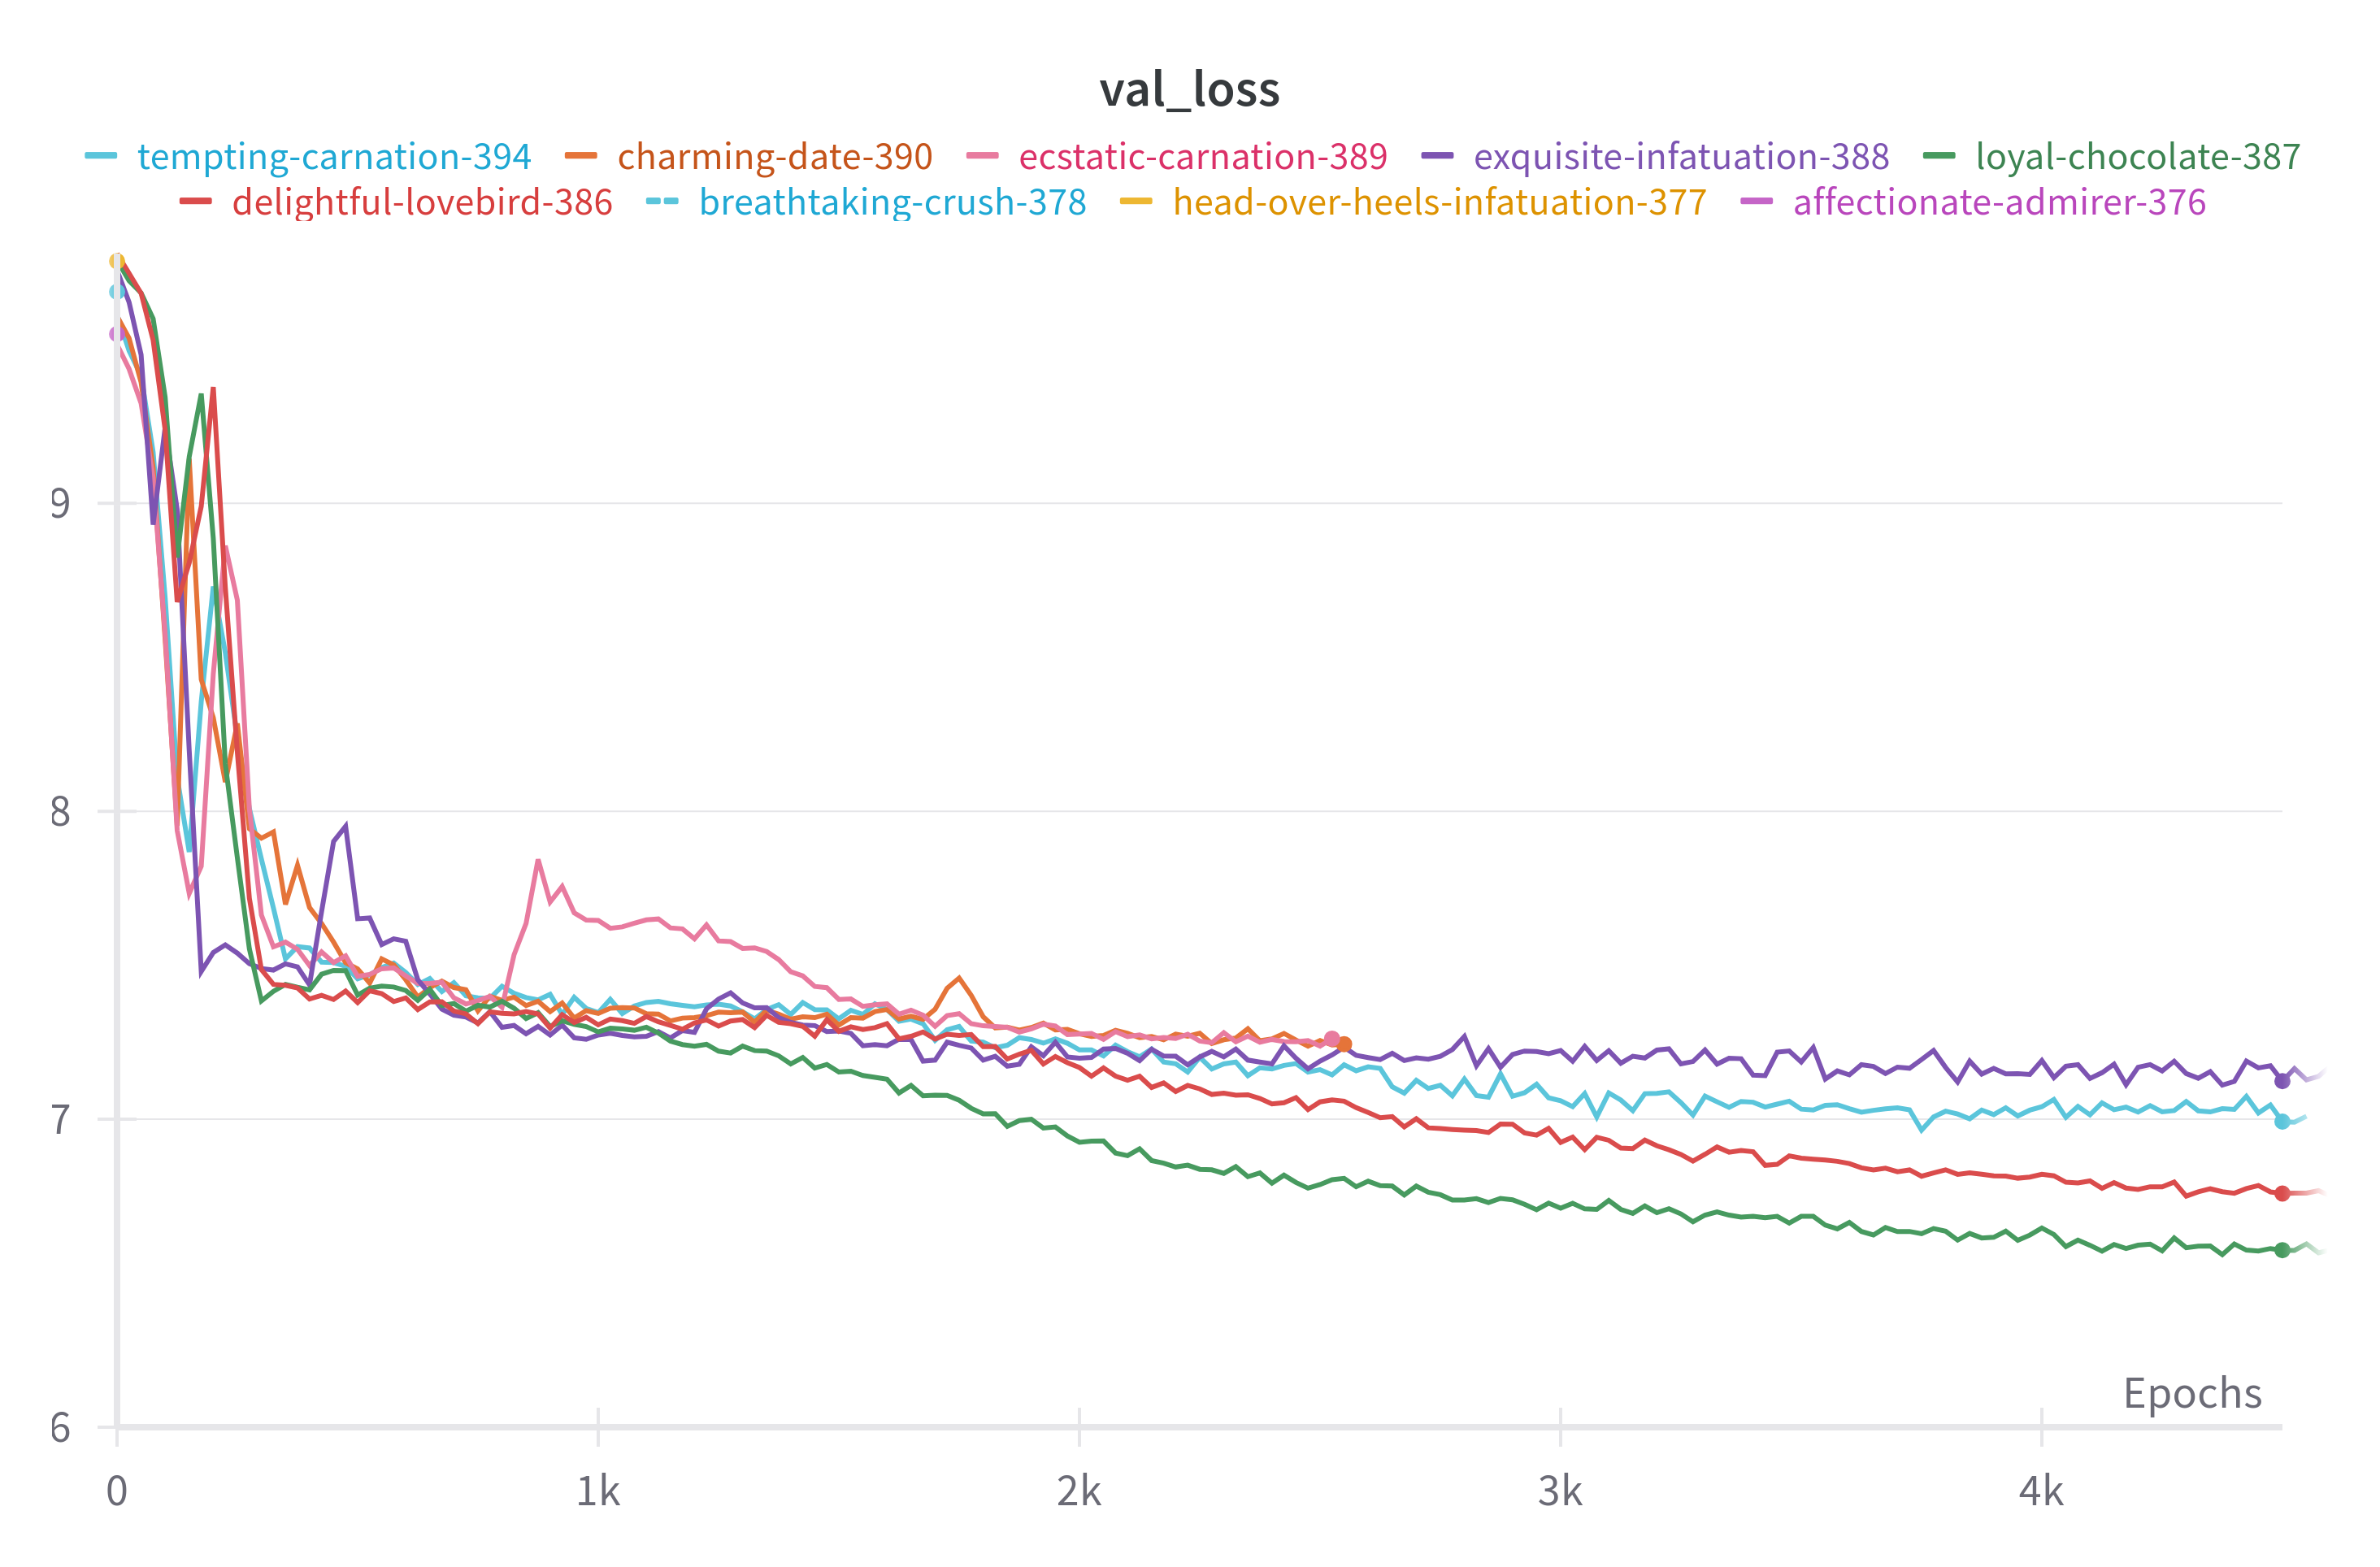
\includegraphics[width=\textwidth]{val_loss.png}
  \caption{Validation Loss}
\end{figure}

\begin{figure}[H]
  \label{fig:train_loss}
  \centering
  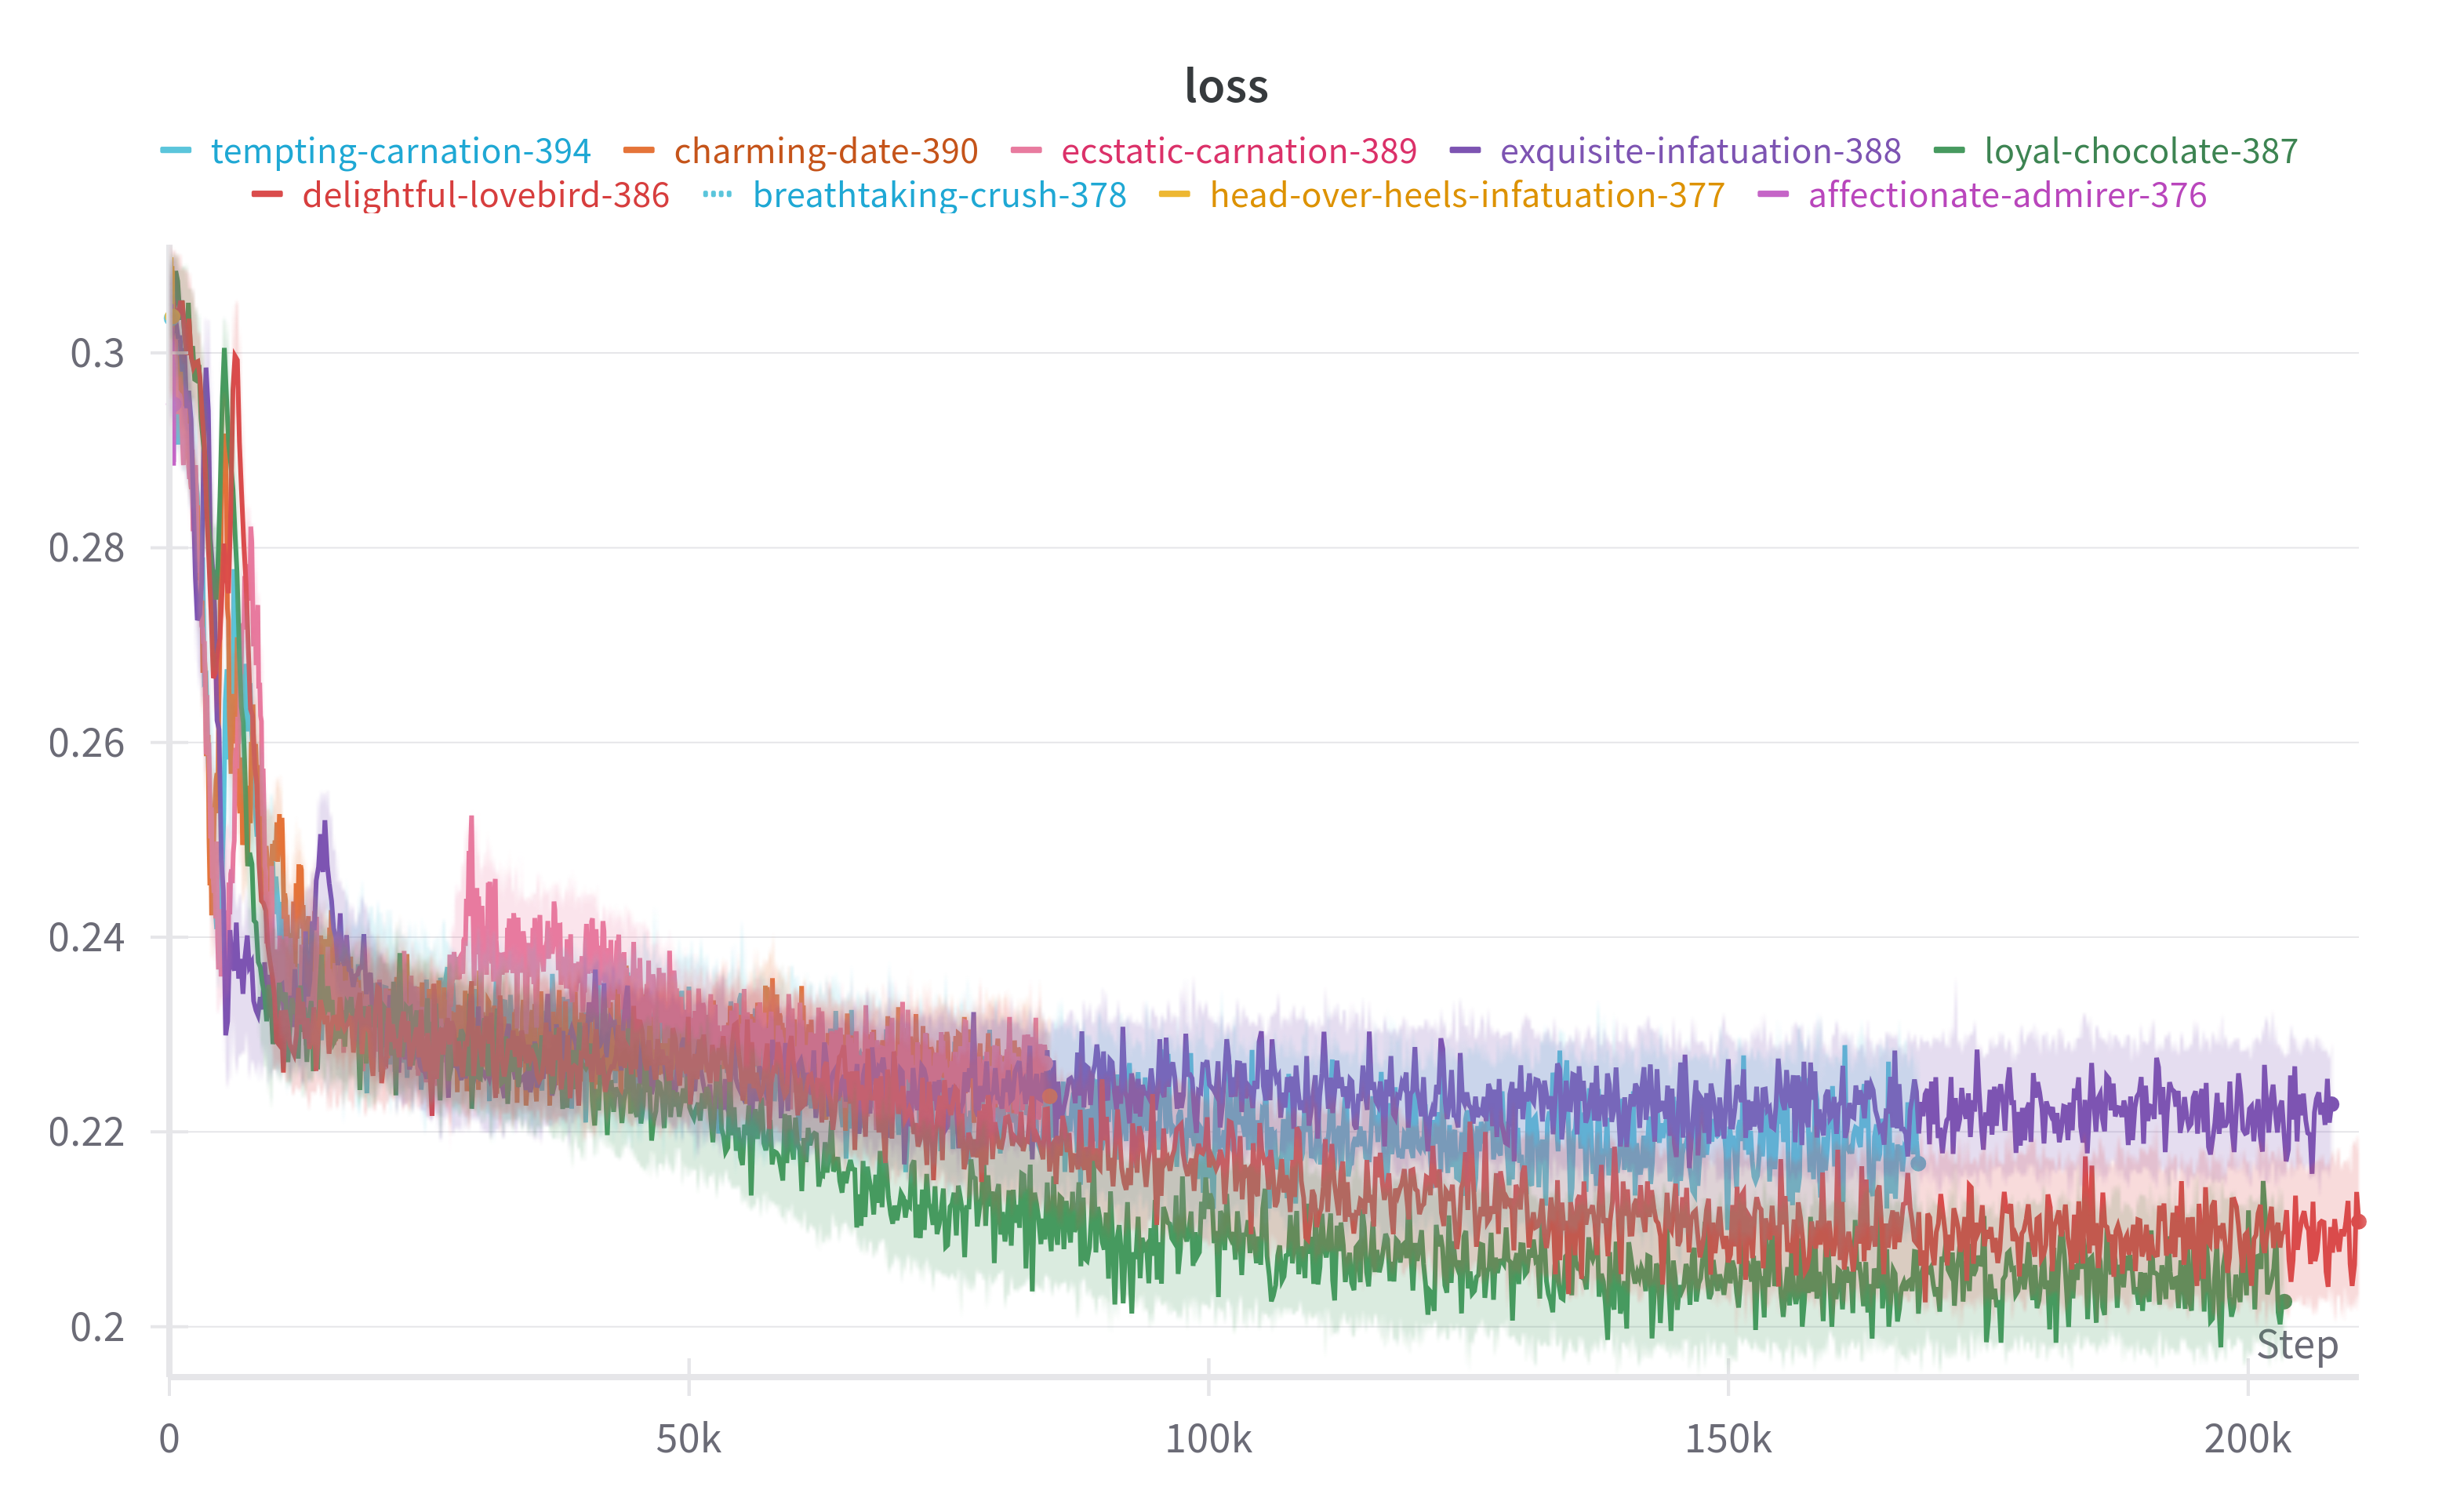
\includegraphics[width=\textwidth]{train_loss.png}
  \caption{Training Loss}
\end{figure}
Our final model is summarized in table (\ref{tab:parameters}).

\begin{center}
    \begin{tabular}{lc}
  \toprule
  \textbf{Parameter} &  \\
  \midrule
  Model & loyal-chocolate \\
  Dropout & 0.35 \\
  intial learning rate & 0.00005 \\
  Heads  & 8 \\
  Embedding Size  & 256 \\
  Layers  & 4 \\
  Context Size & 256 \\
  Vocabulary Size & 4096 \\
  \bottomrule
  \label{tab:parameters}
\end{tabular}
\end{center}
In general we observed that increasing the number of layers, heads or the embedding size did not yield a lower loss.
The context size was chosen given the information we obtained from our token statistics (\ref{sec:token_stats}).
It is important to note again that the way we feed the data into the model does not rely heavily on the most accurate context size given the sequence length distribution of the data.
By randomly selecting data from our input array chances are high that we input two incomplete sequences at once. This is not a problem since the model learns to distinguish between sequences due to the start and end token.


\subsection{Inference Process}

Our inference pipeline generates MIDI sequences based on a given input MIDI file using a trained transformer model. The key steps involved in the process are:

\subsubsection{Model Loading}
We load a pre-trained model from a checkpoint file along with the corresponding vocabulary file. The tokenizer, specified in our the configuration, is initialized to handle MIDI tokenization.
\begin{lstlisting}[language=Python, caption=Loading the pre-trained model and tokenizer]
def load_model(checkpoint_path, vocab_file, batch_size):
    with open(checkpoint_path, mode='r', encoding='utf-8') as weights:
        state_dict = json.load(weights)

    model = GoePT.from_state_dict(state_dict, batch_size=batch_size)
    
    tokenizer = config.tokenizer_name(params=vocab_file)
    return model, tokenizer
\end{lstlisting}

\subsubsection{Tokenization}
The input MIDI files are tokenized using the REMI tokenizer, converting musical events into a sequence of tokens. Special tokens such as Start-of-Sequence (SOS) and End-of-Sequence (EOS) are appended as needed.
\subsubsection{Sequence Generation}
Given a tokenized input sequence, the model generates new tokens autoregressively. The following techniques are applied to enhance the quality of generated sequences:
\begin{itemize}
    \item \textbf{Softmax with Temperature:} Adjusts the sharpness of the probability distribution to control randomness.
    \item \textbf{Top-p Sampling:} Selects tokens from the smallest subset of the vocabulary whose cumulative probability exceeds $p$, ensuring a balance between diversity and coherence. This is explained in more detail in section \ref{sec:6_9}
\end{itemize}

The model generates tokens iteratively, stopping when the End-of-Sequence (EOS) token is encountered or the maximum amount of tokens is reached.

\begin{lstlisting}[language=Python, caption=Generating sequence with EOS stopping condition]
def generate_sequence(model, input_sequence, tokenizer, max_tokens, p, T):
    seq_len = model.context_length
    pad_token = tokenizer.pad_token_id
    sos_token = tokenizer.special_tokens_ids[1]
    eos_token = tokenizer.special_tokens_ids[2]
    
    input_sequence = [sos_token] + tokenizer(input_sequence)[0].ids
    input_sequence = cp.array(input_sequence).reshape(1, -1)
    
    generated_sequence = cp.copy(input_sequence)
    
    for idx in range(max_tokens):
        logits, _ = model.forward(input_sequence, targets=None)
        logits = cp.squeeze(logits, axis=1)  # Transform to 2D shape (batch, vocab)
        
        predictions = softmax_with_temperature(logits, temperature=T)
        next_tokens = top_p_sampling(predictions, p=p)
        
        if next_tokens == eos_token:
            break  # Stop generation when EOS is found
        
        # Append predicted token
        generated_sequence = cp.concatenate([generated_sequence, next_tokens], axis=1)
    
    return generated_sequence.get()  # Move to main memory
\end{lstlisting}

For our purposes

\subsubsection{Post-processing}
After generation, the token sequences are decoded back into MIDI format. Additionally, we apply a monophonic constraint to ensure that only the highest-pitched note is retained in overlapping chords.
This is necessary because we chose not to quantize our MIDI input for tokenization.

\subsection{Top-p Sampling}
\label{sec:6_9}
\subsubsection{Overview}

Before the introduction of Top-p sampling, maximum likelihood decoding and beam search were the standard decoding techniques for generation tasks, but, both of these decoding strategies are prone to generating texts (or melodies) that are repetitive and often end up in loops. Top-p sampling is a decoding strategy for autoregressive language model outputs proposed by \textcite{holtzman2020curiouscaseneuraltext} that solves these issues. To explain it, we will go through the following example:

\begin{figure}[H] % 'h' means here
    \centering
    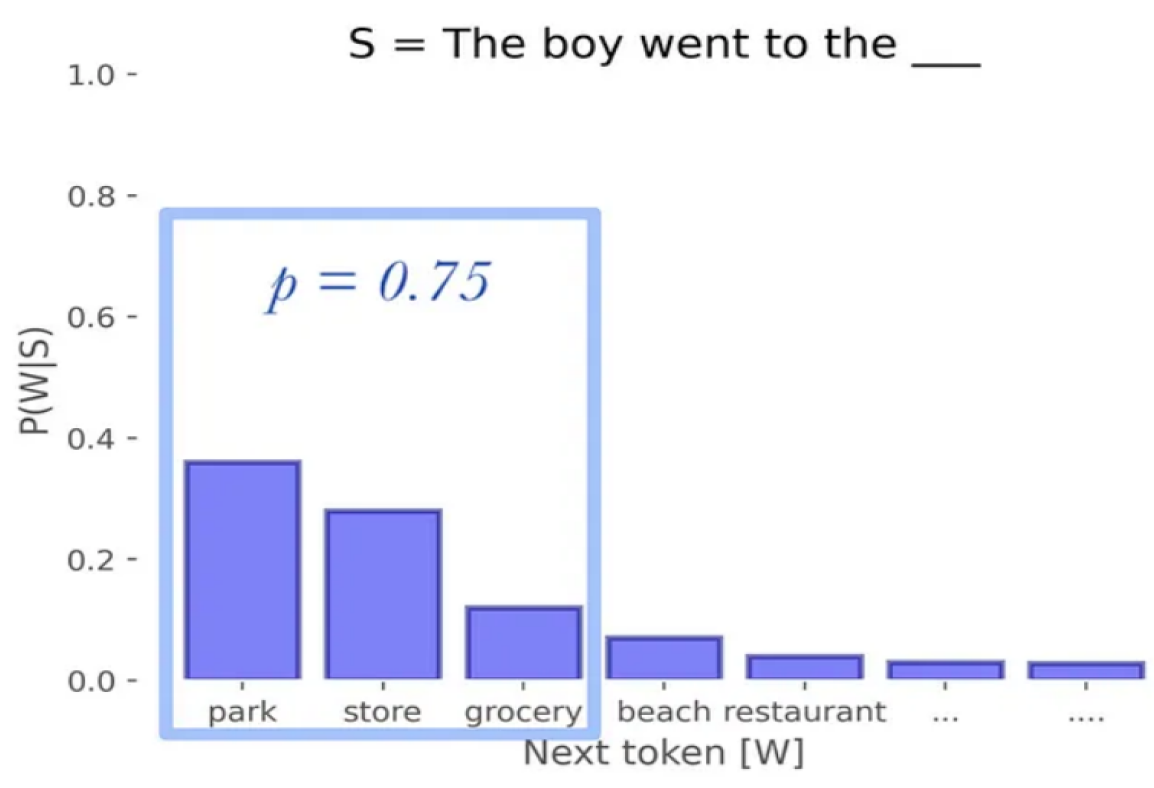
\includegraphics[width=0.6\textwidth]{top p.png} % Adjust width
    \caption{Top-p Sampling, \textcite{TopPWebsite}}
    \label{fig:topp}
\end{figure}

Our task is to predict the next word/token of the sentence S = "The boy went to the ...".

Our model outputs this probability distribution for the next word/token:
$P(park|S) = 0.37, P(store|S) = 0.3, P(grocery|S) = 0.1, P(beach|S) = 0.06$ etc. \newline

The sampling works like this: We set a parameter p. Then we sort the next tokens by their probability from highest to lowest. After that we choose the first k tokens of the list, whose cumulative probability exceeds the threshold p. Our prediction probability for all other tokens we set to 0, the prediction probabilities of the chosen tokens we divide by the cumulative probability, thus rescaling them to be a full probability distribution.\newline

For our example: We choose $p = 0.75$. The first tokens in the sorted list exceeding this threshold are park, store and grocery with cumulative probability $0.77$. These prediction probabilities are rescaled to $P(park|S) = \frac{0.37}{0.77}, P(store|S) = \frac{0.3}{0.77}, P(grocery|S) = \frac{0.1}{0.77}$ and all other token predicition probabibilities are set to 0.\newline

\textit{As an additional note: Top-k sampling is a similar technique except that the sample is taken from the k-highest probability tokens regardless of their cumulative probability. The advantage of top-p sampling is that one avoids the problem of choosing the optimal value of k which can vary depending on the shape of the output distribution and the particular task and dataset.} 

\subsubsection{Implementation}
\begin{lstlisting}
def top_p_sampling(prob_matrix, p=0.2): #Author: both
    batch_size, vocab_size = prob_matrix.shape
    sampled_indices = cp.zeros((batch_size,1), dtype=int)
    
    for i in range(batch_size):
        probs = prob_matrix[i].copy()  # Copy to avoid modifying original data
        
        # Sort tokens by descending probability and get indices
        sorted_indices = cp.argsort(probs)[::-1]
        sorted_probs = probs[sorted_indices]
        
        # Compute cumulative probabilities
        cumulative_probs = cp.cumsum(sorted_probs)
        
        # Find the cutoff where cumulative probability exceeds p
        # Use argmax to find the first index where condition is True; add 1 to include that index
        # If none exceed p, argmax returns 0 (False for all), cutoff becomes 1 (keep the first)
        cutoff = cp.argmax(cumulative_probs > p) + 1
        
        # Slice the top indices and probabilities up to the cutoff
        top_indices = sorted_indices[:cutoff]
        top_probs = sorted_probs[:cutoff]
        
        # Normalize the probabilities
        top_probs /= cp.sum(top_probs)
        
        # Sample from the top distribution
        sampled_index = cp.random.choice(top_indices, size=1, p=top_probs)
        sampled_indices[i] = sampled_index[0]
    
    return sampled_indices
\end{lstlisting}
This is how we implemented the sampling method for our use case (can be found in \textit{Transformer\_Code/CUPY/models/GoePT/Inference.py}). The steps strictly follow the algorithm described in "Overview", any additional explanitions are given in the comments. 
\subsection{Top-p and Temperature Effects on Melodic Outputs}
Lower \textit{top-p} and \textit{temperature} were found to generate more coherent, melody-like sequences. 
This behavior likely arises from the inherent structure of the tokenizer's vocabulary and the probabilistic nature of the decoding process:

\begin{enumerate}
    \item \textbf{Token Distribution Skew:}   \\
    While individual note tokens may have high probabilities during inference, the training data contains a disproportionate number of time-related tokens (tempo, bar, time signature).
    We assume this skew causes these non-melodic tokens to collectively dominate the probability mass, even if no single time token appears in the absolute top ranks.

    \item \textbf{Impact of High p:}  
    When increasing \textit{p}, the sampling pool expands to include lower-ranked tokens. Due to the dataset's structural bias,
    note tokens become statistically "drowned out" by the sheer quantity of tempo/metadata tokens in the expanded pool.
    This results in degenerate sequences overpopulated with non-musical events.

    \item \textbf{Effect of Lower Temperature:}  
    Lower temperature focuses the model on the most likely tokens, which are often notes because they fit the melody best. This helps avoid distractions from less important tokens like tempo markers, keeping the output more musical.

    \item \textbf{Why Lower Settings Work Better:}  
    By reducing both \textit{p} and \textit{temperature}, the decoding process effectively filters out non-essential time tokens, skewing the model toward the smaller subset of tokens that encode pitch, rhythm, and articulation.
    This aligns with the simplicity of monophonic hooks. But choosing \textit{p} and \textit{temperature} to small, the generated sequence will not sound like any recognisable melody.
    In our specific case we used \textit{p}-values of 0.1 to 0.4 and \text{temperate}-values of 0.6 to 0.8.
\end{enumerate}

\section{Conclusion}

% References
\printbibliography



\end{document}
